% Use only LaTeX2e, calling the article.cls class and 12-point type.

\documentclass[12pt,dvipsnames]{article}


%extra packages added during drafting, remove for submission
\usepackage{todonotes}
\usepackage{hyperref}
\usepackage{booktabs}

% Simple little macros to hide and highlight some text:
%\newcommand{\highlight}[1]{{\bf \textcolor{Maroon}{#1}}}
\newcommand{\highlight}[1]{{\bf {#1}}}

%\usepackage{ifthen}
\newif\ifshowoutline
%\showoutlinetrue
\showoutlinefalse
\ifshowoutline
    \newcommand{\outline}[1]{\textcolor{blue}{#1}}
\else
    \newcommand{\outline}[1]{}
\fi


\usepackage{amssymb}
\usepackage{xspace}

\gdef\arcsec{$^{\prime\prime}$}
\def\SNABC{SN Requiem\xspace}

% Users of the {thebibliography} environment or BibTeX should use the
% scicite.sty package, downloadable from *Science* at
% http://www.sciencemag.org/authors/preparing-manuscripts-using-latex 
% This package should properly format in-text
% reference calls and reference-list numbers.


\usepackage{scicite}

\usepackage{times}



% The preamble here sets up a lot of new/revised commands and
% environments.  It's annoying, but please do *not* try to strip these
% out into a separate .sty file (which could lead to the loss of some
% information when we convert the file to other formats).  Instead, keep
% them in the preamble of your main LaTeX source file.


% The following parameters seem to provide a reasonable page setup.

\topmargin 0.0cm
\oddsidemargin 0.2cm
\textwidth 16cm 
\textheight 21cm
\footskip 1.0cm


%The next command sets up an environment for the abstract to your paper.

\newenvironment{sciabstract}{%
\begin{quote} \bf}
{\end{quote}}



% Include your paper's title here

%\title{Requiem for a 10 billion year old supernova } 
\title{A Gravitationally Lensed Supernova with an Observable Decade-long Time Delay}
%\title{A Strongly Lensed Type Ia Supernova with a Decade-Long Time Delay}
%\title{SN Requiem: A Strongly Lensed Type Ia Supernova with a Decade-Long Time Delay}

% Place the author information here.  Please hand-code the contact
% information and notecalls; do *not* use \footnote commands.  Let the
% author contact information appear immediately below the author names
% as shown.  We would also prefer that you don't change the type-size
% settings shown here.


%%%%%%%fill in once decided
% \author
% {John Smith,$^{1\ast}$ Jane Doe,$^{1}$ Joe Scientist$^{2}$\\
% \\
% \normalsize{$^{1}$Department of Chemistry, University of Wherever,}\\
% \normalsize{An Unknown Address, Wherever, ST 00000, USA}\\
% \normalsize{$^{2}$Another Unknown Address, Palookaville, ST 99999, USA}\\
% \\
% \normalsize{$^\ast$To whom correspondence should be addressed; E-mail:  jsmith@wherever.edu.}
% }

% Include the date command, but leave its argument blank.

\date{}



%%%%%%%%%%%%%%%%% END OF PREAMBLE %%%%%%%%%%%%%%%%



\begin{document} 

% Double-space the manuscript.

\baselineskip24pt

% Make the title.

\maketitle 



% Place your abstract within the special {sciabstract} environment.

\begin{sciabstract}
%   The expansion history of the Universe is one of the most fundamental observations leading to the hot big bang model for the origin of the Universe\footnote{Penzias \& Wilson 1965, ApJL, 142, 419}. 
  
  We report the discovery of a quadruply-lensed Type Ia supernova (SN) explosion that will produce a time delay measurement uncertainty of $<1\%$. This unprecedented scenario will enable a unique and highly precise measurement of the Hubble constant from a single lensed SN.  The SN is in an evolved galaxy at $z=1.95$, gravitationally lensed by the massive foreground galaxy cluster MACSJ0138. With three lensed images of the supernova detected in existing observations from the \textit{Hubble Space Telescope} with time delays of order 50 days, this is the most distant multiply-imaged supernova yet discovered.  A fourth image in the component closest to the cluster core is predicted to appear in the year 2035$\pm$2.  Observing the light curve of that future image will provide a time delay precision of $\approx 7$ days over an extraordinary baseline of nearly 20 years. 
  
  

\end{sciabstract}


% In setting up this template for *Science* papers, we've used both
% the \section* command and the \paragraph* command for topical
% divisions.  Which you use will of course depend on the type of paper
% you're writing.  Review Articles tend to have displayed headings, for
% which \section* is more appropriate; Research Articles, when they have
% formal topical divisions at all, tend to signal them with bold text
% that runs into the paragraph, for which \paragraph* is the right
% choice.  Either way, use the asterisk (*) modifier, as shown, to
% suppress numbering.

%\section*{Introduction}



%\todo[inline]{JP: Can edit intro} SN1a play a special role in cosmology, they are standard candles -> led to discovery of DE. High redshift SN-1a provide particularly strong constraints.
%\newline

Observations of Type Ia supernova (SN) explosions have played a key role in mapping the cosmic expansion history, and led to the discovery of dark energy that now appears to be driving an accelerating cosmic expansion rate\cite{riess_observational_1998,perlmutter_measurements_1999, Riess_large_2019}.  Determining the nature of dark energy and how it may evolve over time is a primary goal for the large-scale cosmology experiments of the 2020s \cite{amendola_cosmology_2013,spergel_wide_2015,Ivezic_lsst_2019}.
A series of recent investigations into the expansion rate of the universe (the Hubble-LeM\^aitre constant; $H_0$) have found that measurements from the local universe are significantly different from the value inferred from measurement of the cosmic microwave background (CMB) radiation \cite{Riess_large_2019,aghanim_planck_2018}.  Resolving this tension in $H_0$ measurements may reveal new physics from the early universe \textcolor{red}{Citation here?}, and to do so requires multiple 
independent cosmological probes. 

One promising method uses %time delays of 
gravitational lens systems in which a background
source appears as multiple images that arrive to the observer with relative delays \cite{einstein_lens_1936}.
%, which %for a given lens potential 
When such a strongly-lensed source is variable, one can measure the time delay between any pair of lensed images and derive a ratio of angular diameter distances to the foreground lens and background source. 
This distance ratio is sensitive to cosmological parameters, such as 
%the expansion rate of the universe, 
$H_0$  and the dark energy equation of state, $w$ \cite{refsdal_possibility_1964,coe_cosmological_2009,linder_lensing_2011}.
In recent years this method has been very successfully applied to lensed
quasars \cite{suyu_cosmology_2014,bonvin_cosmograil_2019}, with six high-precision measurements to date \cite{wong_h0licow_2019}. As this sample of time delay lenses grows to several dozen, it is expected to deliver a measurement of $H_0$ with 1\% precision \cite{suyu_cosological_2018}.  

Gravitationally lensed SN with multiple images present an attractive new addition to this field. Most notably, SN exhibit relatively simple photometric behavior, with well-understood light curve shapes and colors---a contrast to the stochastic variation of quasars.  However, the exploration of lensed SN time delay cosmography has been hindered by their rarity.  To date, there have been only two lensed SN observed with multiple images \cite{kelly_multiple_2015,goobar_iptf16geu:_2017}. The first, {\it SN Refsdal}, was a peculiar Type II SN whose image with the longest delay was missed \cite{kelly_SNRefsdal_2016}. The second, {\it SN iPTF16geu}, was a Type Ia SN with short delays that make high precision time delay measurements impossible \cite{dhawan_magnification_2020}. Here we present the discovery 
of a third lensed SN resolved into multiple images: SN Requiem. 


\todo[inline]{put in precise UT dates for HST data and double check newman proposal \href{https://archive.stsci.edu/hst/abstract.html}{(this one?)}}

We discovered SN Requiem using data from the Hubble Space Telescope (HST) program {\it Resolved Quiescent Magnified Galaxies} (REQUIEM, HST-GO-15663, PI:Akhshik). This project targets rare examples of quiescent galaxies that have been magnified by strong gravitational lensing. %These are typically too faint and compact to be resolved even with Hubble, but due to lensing are magnified. This provides a unique opportunity to  understand the still mysterious quenching mechnism. 
The brightest and most spectacular galaxy targeted by REQUIEM
is MRG-M0138, first discovered as a massive red galaxy (MRG) at $z=1.95$ \cite{newman_resolving_2018} behind the massive galaxy cluster MACS J0138.0-2155 \cite{ebeling_macs_2001}.
MRG-M0138 is quadruply lensed by the foreground cluster, which is at $z=0.338$.  
During analysis of REQUIEM observations obtained July 2019 we discovered three point 
sources that were present in archival HST images from July 2016, part of the program 
that originally discovered the MRG-M0138 galaxy (HST-GO-14496; PI:Newman). 
Each point source is within 5 arcseconds of one of the four MRG-M0138 images.  None of the
three point sources are present in the REQUIEM HST data in 2019 (Fig \ref{fig:layout}). We infer that 
the point sources are multiple images of a single astrophysical 
transient in MRG-M0138, most likely a SN. Hereafter we call this multiply-imaged transient {\it SN Requiem}.

To construct a lens model for the MACS J0138.0-2155 cluster we used the publicly available {\tt Lenstool} software \cite{jullo_bayesian_2007, kneib_lenstool_2011} to model the mass distribution in the cluster core as the combination of a cluster scale and multiple galaxy scale potentials.  To avoid unintended bias, we kept the lens model development completely separate from the analysis of the SN.  Only upon independent completion of both were the results combined for the analysis described here.  The input model constraints are the positions and redshifts of the MRG-M0138 galaxy at $z=1.95$ (both the central light peak and the SN location in each image) as well as a multiply-imaged background 
galaxy at $z=0.766$, both having secure spectroscopic redshifts.  
From this model we derive estimates for the lensing magnification and time delay of each of the SN images, including the predicted fourth image (Tab 1).
The lensing model predicts that the SN should appear in the fourth MRG-M0138 image in 20XX+/-X., with a magnification of X. A fifth image will also appear in 20XX+/- but this will be demagnified and likely not observable.

%The range of possible transients for Requiem is broad, encompassing normal SNe, superluminous SNe (galyam luminous 2019), fast transients (berger fast 2013, drout rapidly 2014), and even gravitational microlensing events (rodney two 2018, kelly extreme 2018). 
To realize the cosmological promise of SN Requiem 
we need to estimate the age of each SN image, which in turn constrains the lensing time delays. For this
goal, it is valuable to have a firm determination of the transient’s class. Expected time delays and magnifications from the lens model exclude any of the various rapidly evolving and low-luminosity stellar transient classes, strongly suggesting that it is a SN. The first-order SN distinction remaining is between a Type Ia SN---the explosion of a white dwarf star in a binary system---and a core collapse SN (CCSN)---the end-point of a star with mass $\gtrsim 10 M_{\odot}$. 
The properties of the host galaxy can inform this classification because CCSN are limited to galaxies with young stellar populations. Limits on the specific star formation rate and age for this host, MRG-M0138, show it to be a high-mass but very quiescent and evolved galaxy, %($\log(M_*/M_\odot)=11.7\pm0.2; )$ , 
unlikely to retain any significant population of high-mass stars \cite{newman_resolving_2018}. Based on observed properties of the host galaxy alone, we find a 75\% probability that Requiem is a Type Ia SN (see supplementary text). Adopting the lens model magnifications for the three observed SN images (Table S2) the position of each SN image in color-magnitude space (Fig \ref{fig:class}) provides more classification leverage, yielding p(Ia)=\textcolor{red}{XX}. By also including the measured time delays, we can treat the three SN images effectively as three points on a common SN light curve, and we find p(Ia)=\textcolor{Orange}{YY} (Fig \ref{fig:class}).
%This is corroborated by the limited data available for the transient. In color -magnitude space it displays best agreement with the Type Ia population (Fig 1). 
An improved classification can be achieved with spectroscopy and multi-band photometry upon arrival of the fourth image.


%The galaxy has very low SFR=XX and based on stellar ages stopped forming stars ~X.X Gyr earlier. This is a proto typical early type galaxy progenitor.

%%%%%% ORIGINAL Classification text
% To evaluate the age of each transient image (and therefore constrain the lensing time delay between images), it is valuable to have a firm determination of the transient's class.  The range of possible transients is broad, encompassing normal SNe, superluminous SNe \citep{galyam_luminous_2019}, fast transients \citep{berger_fast_2013, drout_rapidly_2014}, and even gravitational microlensing events \citep{rodney_two_2018,kelly_extreme_2018}.  Identifying the transient type makes it possible to use the well-developed library of spectrophotometric SN models \citep[e.g.][]{kessler_models_2019} for the time delay measurement. 
%  The first-order distinction that is most important is between a Type Ia SN--understood to be the explosion of a white dwarf star in a binary system--and core collapse SN (CCSN)--the end-point of a star with mass $\gtrsim 10$M$_{\odot}$.  Given the limited data available for this transient, we will not attempt a more fine-grained classification, though in principle that could be achieved with spectroscopy and multi-band photometry upon arrival of the final image.  
 


% As a first step, we can use inferences from the lens model to establish a strong prior against any of the various rapidly evolving and low-luminosity stellar transient classes.  
% The expected time delays between the images are $\sim100$ observer-frame days, 
% but we see that three images of the transient are visible simultaneously.
% From this we can infer that the visibility time of the transient in the $z=1.95$ rest-frame must be at least $\sim$30 days. 
% Similarly, with expected magnifications in the vicinity of $\mu\sim10$, the measured apparent magnitudes near 23 AB mag translate to a rest-frame absolute magnitude near $M_B \sim-19.5$ mag (too bright to be a nova, luminous blue variable, or other low-luminosity stellar transient).
% Taken together, these indicators strongly suggest that the transient is a supernova (SN). 

% Although we have invoked the lens model in this analysis, note that the inferences are not strongly dependent on the specific lens model predictions.  To make the observed transient images consistent with a fast or low-luminosity transient, the time delays and/or magnifications would have to be changed by more than a factor of 2.  In the analysis to follow, we will work under the assumption that the transient is a SN. 

% \subsection{Host galaxy properties}
% \label{ss:host}

% We first seek to classify this transient {\it circumstantially}, using measured properties of the host galaxy stellar population to infer the type. Although Type Ia SNe are found in all types of galaxies, CCSNe are limited to galaxies with relatively young stellar populations.  We can therefore infer some information about the SN type using the observed host properties combined with knowledge of the relative rates of Type Ia and CCSNe in different stellar populations \citep{mannucci_rates_2005,foley_classifying_2013}.  In the case of the host galaxy MRG0138, we have very stringent limits on the star formation rate. This galaxy is a high-mass but very quiescent galaxy, with a specific star formation rate of $\sim10^{-11.3}$ yr$^{-1}$  and a stellar population that is well-matched by an exponential star formation history with an age of $1.4$ Gyr \cite{newman_resolving_2018}.  The massive stars that end as CCSN explosions have main-sequence lifetimes of $\lesssim 40$ Myr,  making it highly unlikely that MRG0138 retains any significant population of massive stars \SR{this should be revised, b/c of total mass.  Focus instead on the relative probability. as discussed on telecon}


% Discussion from Newman et al. \citep{newman_resolving_2018-1}.

% Conclusion: the host is a red-dead elliptical. It is most likely a Type Ia SN.

% \subsection{Classification from Color and Brightness}
% \label{ss:lightcurve}

% Figure~\ref{fig:colormag} shows the location of \SNABC in color-magnitude space, comparing the de-magnified apparent F160W magnitude against the observed F105W-F160W color.  
% For a source at $z=1.95$ the F160W band is centered near 5400 \AA, approximately corresponding to the Bessell V bandpass, while the F105W-F160W color approximates a U-V color. 
% As shown in Figure~\ref{fig:colormag}, the observed photometry for \SNABC is fully consistent with the expected color and magnitude of a Type Ia SN at $z=1.95$, after correcting for lensing magnification using the $\mu$ values from Table~\ref{tab:model_evidence}.  The magnification-corrected photometry is inconsistent with Type II SNe, which are fainter and more blue. \SNABC is marginally consistent with the CCSN Type Ib/Ic sub-class, although the image 2 point falls outside of the 95\% confidence region for that population.  

% The right panel in Figure~\ref{fig:colormag} shows that the three data points are also consistent with the expected time-dependence  of a Type Ia SN in this color-magnitude space. Visualizing the changing color and brightness of a SNIa at $z=1.95$ in the F105W and F160W bands, we see that it  would intersect image 2 near peak brightness and approach the image 1 and 3 photometry at roughly 80 observer-frame days after peak.  

% Taken together, this evidence reinforces the conclusion that \SNABC is most likely a Type Ia SN.  Although we have to adopt a magnification correction 
% from a lens model, this conclusion is not sensitive to the choice of lens model.  Every lens model we have evaluated locates \SNABC's un-magnified position squarely within the Type Ia region of color-magnitude space.  
% Dust is also not a confounding factor here.  The simulations used to generate the contours in Figure~\ref{fig:colormag} include dust extinction at the source plane.  If a significant screen of dust exists in the lens plane, this would have the effect of making the SN appear dimmer and more red, so correcting for that extinction would move the \SNABC requiem points upward and leftward on this plot, causing it to be even more strongly associated with the Type Ia region. 

% \SR{TODO: add an appendix explaining the sims}



\outline{
Multiple lensed transient or varying sources can be used to constrain cosmology, through timedelay measurements.  Many quasars lensed by galaxies known, provide some of the most accurate measurements of H0.  Possibly in dissagremment with CMB }
\newline
\newline
\outline{
Refsdal proposed multiple lensed SN as means of constraining cosmology. A few have been observed (list), most famously the Refsdal SN, a Type II at z=1.5 lensed by a cluster, missed one image, observed 2 and predicted a fourth that was later observed
}\newline
\newline
\outline{
Requiem is a hubble project that target rare examples of quiescent galaxies, that have been magnified by gravitational lensing. These are typically too faint and compact to be resolved even with Hubble, but due to lensing are magnified. This provides a unique opportunity to  understand the still mysterious quenching mechnism. 
The brightest and most spectacular target of REQUIEM, first discovered by Newman in 2016 is RGM0138, is a z=2.X, logM=XX quiescent galaxy quadruply lensed by a cluster at z=0.X. The galaxy has very low SFR=XX and based on stellar ages stopped forming stars ~X.X Gyr earlier. This is a proto typical early type galaxy progenitor.
}
\newline
\newline
\outline{
During analysis of the REQUIEM observations obtained  July 2019 we discovered a new pointsource close to three of the four images, which was not there in the original Hubble images taken in July 2016 (PI Newman), when the system was first discovered (Fig \ref{fig:layout}). 
}
\newline
\newline

\outline{
\todo[inline]{JP: I'll fill this in from the old text, then SR and/or KO work on this classification section} The SN has different colors and brightness in the three observed images. This is expected as SN evolve in brightness and color with time, and the three images represent different times on the supernova light curve, due to the different time delays of the different images. Fig \ref{fig:class} shows the colors and magnitudes expected for different types of SN lightcurves. The observations classify the explosion as a Type Ia, when the magnifications from the lensing model is taken into account. This is consistent with the host galaxy being an evolved early type (void of O and B stars). Using the absolute magnitude, $M_K$, and color, $B-K$, of the host, there is about 75 percent probability that the object is of type Ia (citation to https://arxiv.org/pdf/1309.2630.pdf).
}
\newline
\newline
\outline{
\todo[inline]{JP: Need Johan to fill in this section, or give details for us to fill it in} The lensing model is derived using the lenstool software, constrained by XX spectroscopically confirmed lensed images, and scaling relation for the cluster galaxies, as well as local pertubers .... (johan)
}
\newline
\newline
\outline{
\todo[inline]{JP: I'll fill this in + Johan lens model stuff, this will include time delay/magnification constraints from SNTD} In addition to the relative magnifications of the individual images, the lensing model predicts relative timdelays between the images. These are are XXX in a greement with the observed colors evolution in Fig 2 providing confidence in the accuracy of the lensing model. The lensing model predicts that the SN should appear in the fourth image in 20XX+/-X., with a magnification of X. A fifth image will also appear in 20XX+/- but this will be demagnified and likely not observable.
}
\newline
\newline
\outline{
This is the second highest redshift SNIa, it is the first one that where we observe it from the appearance of the first image to the last (Refsdal had an image that appeared Xyears before it was first dicovered), and it it the one with the longest (predicted) timedelay.  Add here other properties that make the system unique.
}
\newline
\newline
\outline{
\todo[inline]{JP: Can edit time delay/cosmo section} Due to the long timedelay baseline, the sensitivity to cosmology is exceptional, and the precision with which cosmological parameters can be constrained is limited only by the precision of the lensing model. Assuming that H0 is determined from other methods when the fourth image appears in 20XX Fig 3 shows that this single system will have provide comparable (and complementary) constraints as those expectede from tens of lensed supernova in planned LSST and WFIRST cosmological surveys. At that time JWST will likely be in the past but we will have E-ELT, and XXX.. which will allow for cool science such as...
}

The color of a SNIa evolves substantially over its lifetime as the photosphere expands and cools, revealing different layers of the expanding shell and driving episodes of recombination \cite{woosley_type_2007,kasen_type_2009}. Since the phenomenon of gravitational lensing in general is achromatic, this color evolution makes it possible to derive an age constraint that is largely independent of the lens model.\todo{add a lens-model-independent precision statement?}  Combining this information with magnification constraints from the lens modeling helps break parameter degeneracies, yielding the measured delays in Table 1. 
Remarkably, the ages of image 1 and 3 are constrained to better than $\pm$20 days, despite having only a single epoch of photometric data.   These uncertainties may be 
further reduced when the future fourth image is observed with high-precision, multi-epoch photometry.  Such a light curve will pin down the intrinsic SN light curve parameters that are shared by all images.
%These constraints represent an upper limit on the age (and therefore time delay) uncertainties, but they would still deliver an uncertainty of $\sim0.3\%$ on the predicted $\sim6000$ day delay. While already dwarfed by the expected lens model uncertainty, constraints on the intrinsic SN light curve parameters gained from exquisite photometry of the future fourth image of Requiem could improve this even further. 

Future large scale surveys such as the Vera C. Rubin Observatory 
%Legacy Survey of Space and Time (LSST) 
and the Nancy Grace Roman Space Telescope will observe dozens to hundreds of lensed SN over their duration \cite{oguri_gravitationally_2010,goldstein_rates_2019,wojtak_magnified_2019}. However, many of these lensed SN will require follow-up resources and all will have significantly shorter delays (and therefore higher relative uncertainties) than SN Requiem. In Figure \ref{fig:cosmo} we imagine a scenario in which scarce follow-up resources could be used to observe $\sim5$ objects. We compare the cosmological constraints obtainable from small samples of SN representative of those expected from the Rubin Observatory and the Roman Space Telescope, with ``Requiem-Like'' SN. 


Because of the unusually large ratio of source to lens redshift, the constraints on dark energy equation of state parameters ($w_0$, $w_a$) from the Requiem-like sample are nicely complementary to the samples accessible to the wide-area Rubin Observatory and Roman Space Telescope surveys. The extraordinarily long time delays of cluster-lensed SNe like SN Requiem also deliver significantly better time delay precision, with comparable observational cost.  
Such a sample could be developed with regular monitoring of cluster-scale lenses.  As SN Requiem has shown, even a single epoch of photometric data at the time of detection may be sufficient to provide the necessary anchor point for this promising cosmological tool.  





% Your references go at the end of the main text, and before the
% figures.  For this document we've used BibTeX, the .bib file
% scibib.bib, and the .bst file Science.bst.  The package scicite.sty
% was included to format the reference numbers according to *Science*
% style.

%BibTeX users: After compilation, comment out the following two lines and paste in
% the generated .bbl file. 
\clearpage
\begin{figure*}
    \centering
    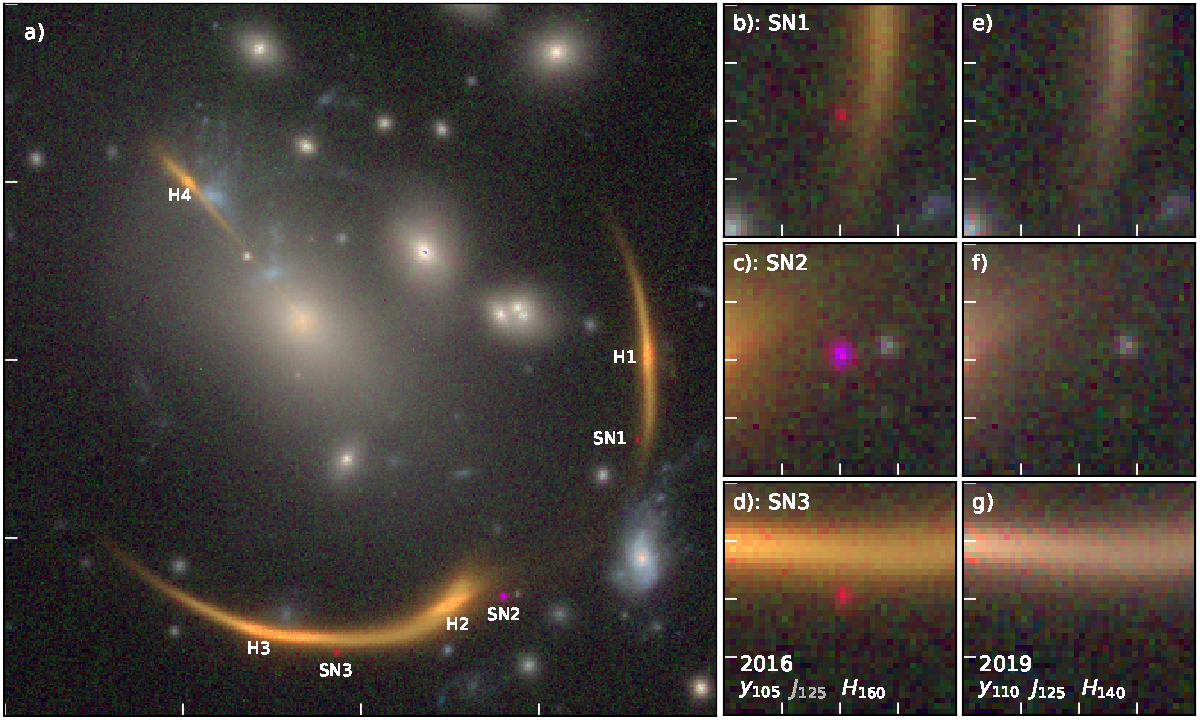
\includegraphics[width=0.9\textwidth]{Paper/Figures/fig1_layout.pdf}
    \caption{Overview of the field around the center of the MACSJ0138 cluster field and the locations of the lensed host (H1--4) and \SNABC (SN1--3) images. The wide-field view in $a)$ is 40\arcsec\ on a side with ticks indicating 10\arcsec\ intervals.  Panels b--g) show 4\arcsec\ cutouts around the lensed SN images with 1\arcsec\ ticks.  The three-color images are generated from the WFC3/IR filters as indicated; panels $b$--$d$ show the imaging from July 2016 where the SN was visible and $e$--$g$ show the later imaging from July 2019 where the the SN has faded away.  All panels use the late-epoch F125W imaging for the green channel.  Nevertheless, it is immediately clear that the SN2 image is substantially bluer than the other two, which we use to constrain the transient classification as a likely Ia supernova explosion.}
    
    \label{fig:layout}
\end{figure*}
\clearpage
\begin{figure}[h]
    \centering
    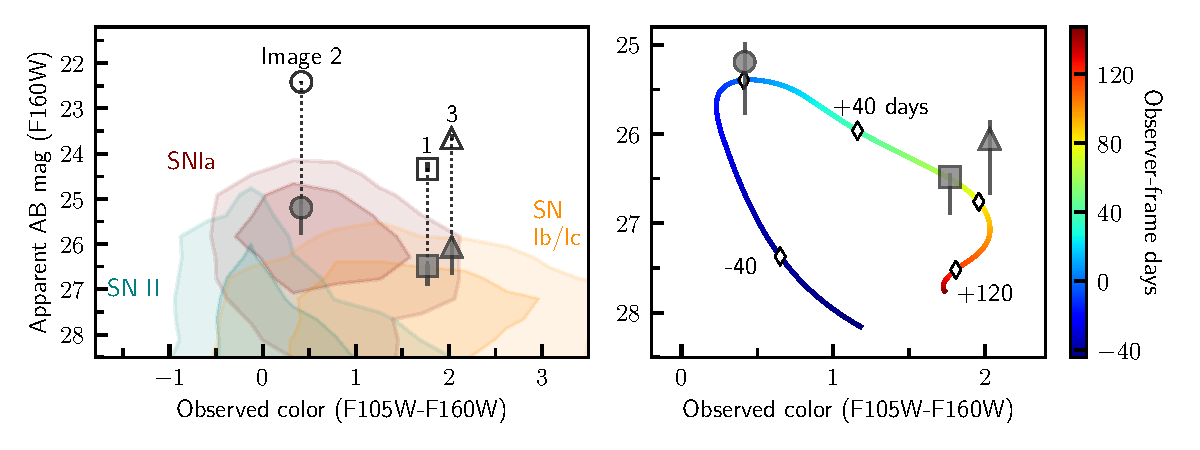
\includegraphics[width=\textwidth]{Paper/Figures/classification_contours_timeline.pdf}
    \caption{Classification information for \SNABC based on its position in color-magnitude space. (left) Contours show the population distributions for normal SNe of Type Ia (red), Type Ib/Ic (gold), and Type II (green).  These population contours are drawn to enclose 68\% (interior solid lines) and 95\% (exterior shaded regions) of each SN population.  Each SN sub-class was simulated at $z=1.95$, and samples from their expected light curves were drawn uniformly in time. Open markers show the observed photometry of the SN. Dotted vertical lines mark the magnification correction based on the lens modeling, terminating in closed markers with error bars that show the magnitude uncertainty, which is dominated by the lens modeling uncertainty.  (right) The evolution of a Type Ia SN at $z=1.95$ in observed color-mag space is shown by a colored line, with the color indicating SN age in observer-frame days relative to peak brightness.  White diamonds correspond to the times labeled on the colorbar at right. An interactive 3-D version of this figure is available online at \href{https://plot.ly/~jpierel/6/#/}{https://plot.ly/~jpierel/6/#/}
    \label{fig:class}
    }
\end{figure}

\clearpage
\begin{figure}
    \centering
    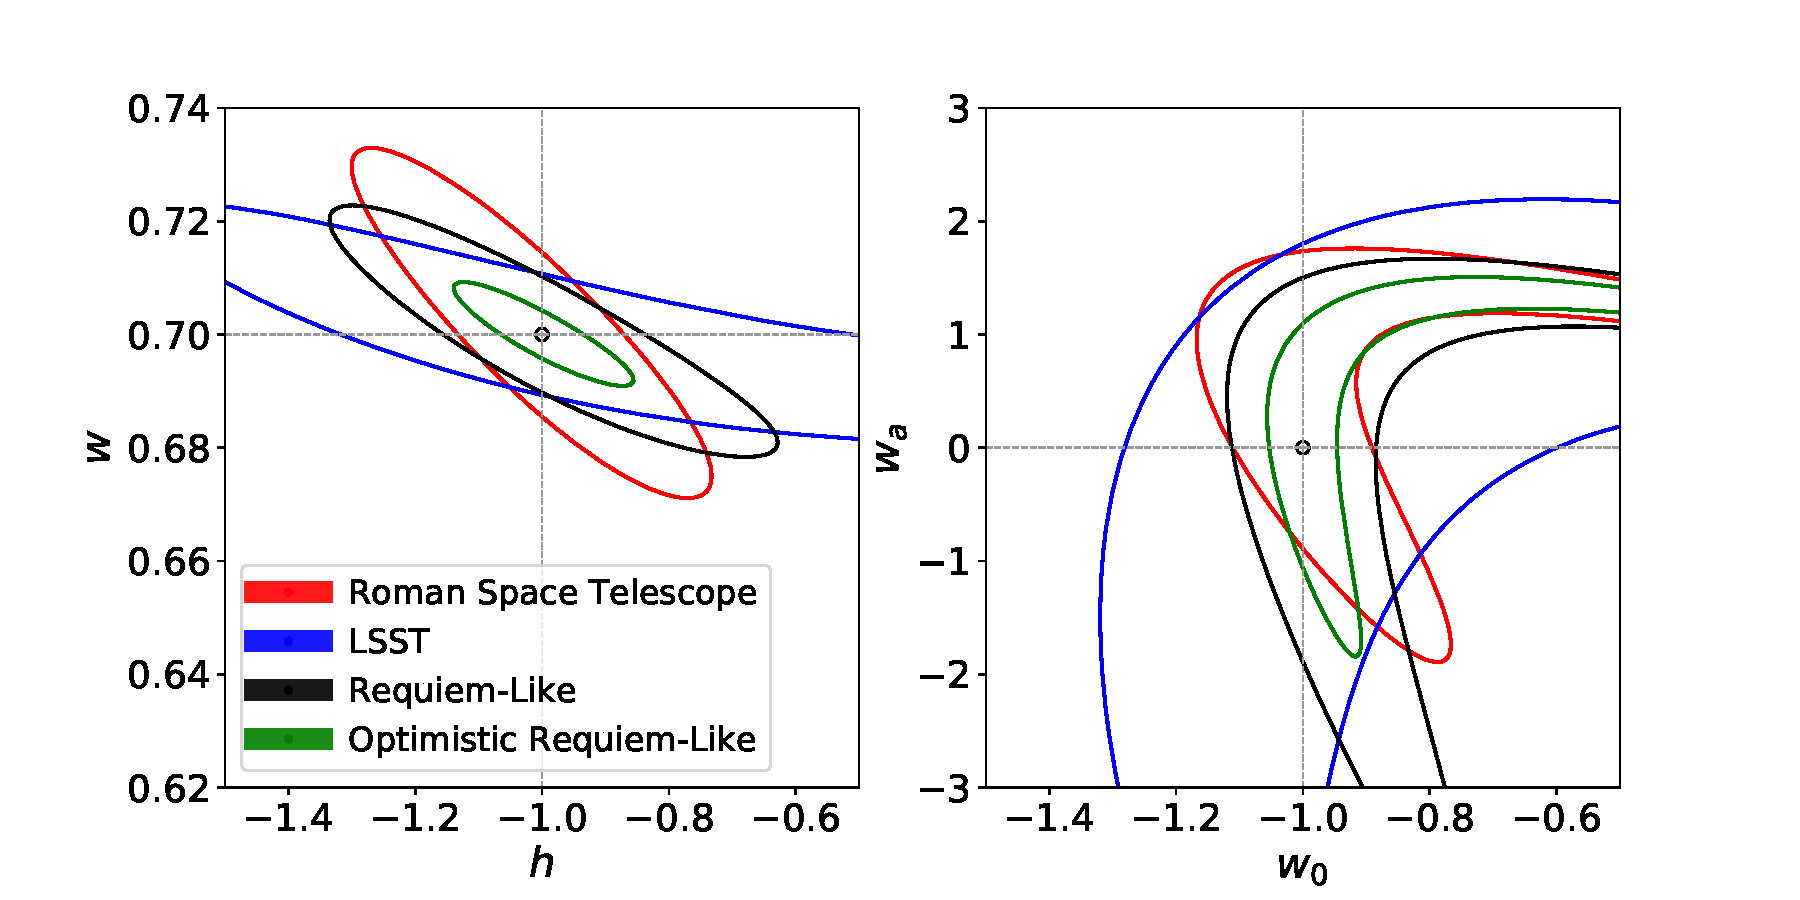
\includegraphics[width=\textwidth]{../Figures/snrequiem_hw_w0wa_apples_to_lsst_ngrst.pdf}
    \caption{ \todo[inline]{replace caption for new figure}The unusual sensitivity of SN Requiem to dark energy equation of state parameters ($w_0, w_a$). Contours show the 1$\sigma$ confidence region for a typical sample of lensed SNIa time delays from LSST (blue) and WFIRST (red) compared to SN Requiem (magenta), which is shown for assumed uncertainties on the lens potential of 5\% and 2\%. Dashed lines and the white marker show the input values of $w_0=-1$, $w_a=0$ that were used for this simulation. In order to isolate the $w_0, w_a$ dependence, all contours are constructed assuming perfect knowledge of $H_0$, $\Omega_{m,0}$ and $\Omega_{\rm de,0}$.  SN Requiem could be highly complementary to the LSST+WFIRST lensed SN sample, due to its unusual combination of a relatively low-redshift lens ($z=0.338$) and high-redshift source ($z=1.95$). This single SN could deliver constraints on dark energy equation of state parameters comparable to several dozen SNe with shorter and less precise  time delays.}
    \label{fig:cosmo}
\end{figure}

\clearpage

\begin{table}
\centering
\begin{tabular}{crr|rrrr}
    \multicolumn{1}{c}{}&
    \multicolumn{2}{c}{\textbf{Photometry}}&\multicolumn{2}{c}{\textbf{Lens Model}}\\
    %\multicolumn{1}{c}{}&\multicolumn{1}{c}{}\\
    \multicolumn{1}{c}{\textbf{Image}} &\multicolumn{1}{c}{\textbf{Age}} &\multicolumn{1}{c}{$\mathbf{t_i-t_2}$}&\multicolumn{1}{c}{$\mathbf{\mu}$}
    &\multicolumn{1}{c}{$\mathbf{t_i-t_2}$}\\
    
\midrule

\textit{1}  &$79.10^{+45.56}_{-11.76}$&$91.31^{+62.49}_{-23.36}$ &8.942&103.6\\
\textit{2} & $-16.67^{+19.14}_{-13.10}$&-- \ \ \ \ \ \ \ \ \  & 18.48&-- \ \ \ \ \\
\textit{3} &$80.46^{+20.10}_{-9.84}$&$92.60^{+37.28}_{-21.76}$ & 13.257&153.8\\
\textit{4} &-- \ \ \ \ \ \ \ \ \ &-- \ \ \ \ \ \ \ \ \ &1.137&5980.4\\


\end{tabular}
\caption{\label{tab:time_delays}Time Delays}
\end{table}

\bibliography{references}

\bibliographystyle{Science}





\section*{Acknowledgments}

The Cosmic Dawn Center of Excellence funded by the Danish National Research Foundation under grant No. 140.

%Here you should list the contents of your Supplementary Materials -- below is an example. 
%You should include a list of Supplementary figures, Tables, and any references that appear only in the SM. 
%Note that the reference numbering continues from the main text to the SM.
% In the example below, Refs. 4-10 were cited only in the SM.     

\clearpage
\section*{Supplementary materials}
Materials and Methods\\
Supplementary Text\\
Figs. S1 to S10\\
Tables S1 to S2\\
References \textit{(4-10)}
\clearpage
\setcounter{table}{0}
\renewcommand{\thetable}{S\arabic{table}}

\setcounter{figure}{0}
\renewcommand{\thefigure}{S\arabic{figure}}
% For your review copy (i.e., the file you initially send in for
% evaluation), you can use the {figure} environment and the
% \includegraphics command to stream your figures into the text, placing
% all figures at the end.  For the final, revised manuscript for
% acceptance and production, however, PostScript or other graphics
% should not be streamed into your compliled file.  Instead, set
% captions as simple paragraphs (with a \noindent tag), setting them
% off from the rest of the text with a \clearpage as shown  below, and
% submit figures as separate files according to the Art Department's
% instructions.

\section*{Materials and Methods}
%\todo[inline]{I'm not really sure what this section is for, or if we need it (commented out is the description from science about what this should be)}
% The materials and methods section should provide sufficient information to allow replication of the study. It should be cited at relevant points in the text using a citation number that refers to a note in the reference list that reads “Materials and methods are available as supplementary materials at the Science website.” Study design should be described in detail and descriptions of reagents and equipment should facilitate replication (for example source and purity of reagents should be specified, there should be evidence that antibodies have been validated, and cell lines should be authenticated). Clinical and preclinical studies should include a section titled Experimental Design at the beginning of materials and methods in which the objectives and design of the study, as well as prespecified components, are described. Statistical methods must be described with enough detail to enable a knowledgeable reader with access to the original data to verify the results. The values for N, P, and the specific statistical test performed for each experiment should be included in the appropriate figure legend or main text.  Please see our editorial policies for additional guidelines for specific types of studies as well as further details on reporting of statistical analysis. For papers in the life sciences that involve a method that would benefit from the publication of a step-by-step protocol, we encourage authors to consider submitting a detailed protocol to our collaborative partner Bio-protocol.

\subsection*{Observations of the SN and Lensing System}

The observations of MRG0138 used in this work are  summarized in Table \ref{tab:observations}.   For this work, all HST observations were processed using the {\tt Drizzlepac} software utilities \cite{gonzaga_drizzlepac_2012}, aligned to a common astrometric reference frame and resampled to a pixel scale of 0.1 arcseconds per pixel.  We then identified isolated and unsaturated stars in each image and used them to create an effective point spread function (ePSF) with $4\times$ oversampling, using the {\tt photutils} package from the {\tt astropy} software suite \cite{astropy_citation_needed}.   To measure the SN photometry we followed two tracks.  As our primary method we performed ePSF-fitting directly on the F105W and F160W images where the SN was apparent.  This ePSF fitting allowed for a fixed background flux to account for both the sky brightness and the background light of the cluster and host galaxy.  
As a second approach, we created ``pseudo-difference images'' by rescaling the later F110W and F140W images collected in 2019 (in which the SN is not present).  The transmission functions of the F110W and F140W filters are broader than F105W and F160W, and do not strictly overlap in wavelength.  The optimal scaling factor to produce a clean subtraction therefore depends on the spectral energy distribution of the source.  We set the scaling to 0.62 and 1.17 for F110W-to-F105W and F140W-to-F160W, respectively.  These values produced visually clean subtractions of the SN host galaxy MRG0138---meaning that they minimize the residual flux from MRG0138 left behind in the pseudo-difference images.  We then performed ePSF fitting on the SN in each pseudo-difference image, using the same ePSF model as before.   Both sets of photometry agree to within one standard deviation.  The reported photometry in Table~\ref{tab:photometry} are the first  measurements, collected directly from the unsubtracted images.

\begin{table}[h]
\centering
\begin{tabular}{ccccccr}
    \multicolumn{1}{c}{Telescope} & \multicolumn{1}{c}{Instrument} & \multicolumn{1}{c}{$\lambda_\mathrm{obs}$} & \multicolumn{1}{c}{Observation Date} & \multicolumn{1}{c}{MJD} & \multicolumn{1}{c}{SN} & \multicolumn{1}{c}{Exp. Time (s)}\\

\midrule
\textit{Spitzer} & IRAC      & $3.6\,\mu\mathrm{m}$      & 2016-03-15 03:44:04 & 57462.1556 &   & 212 \\ % AOR r58785536
\textit{Spitzer} & IRAC      & $4.5\,\mu\mathrm{m}$      & 2016-03-15 03:44:04 & 57462.1556 &   & 241 \\
\textit{HST}     & ACS/WFC   & F555W                     & 2016-06-03 21:50:43 & 57542.9102 &   & 5214 \\
\textit{HST}     & WFC3/IR   & F160W                     & 2016-07-18 23:14:50 & 57587.9686 & + & 1611 \\
\textit{HST}     & WFC3/IR   & F105W                     & 2016-07-19 00:43:47 & 57588.0304 & + & 3611 \\ 
\textit{Spitzer} & IRAC      & $3.6\,\mu\mathrm{m}$      & 2016-10-13 14:35:13 & 57674.6078 &   & 468 \\ % AOR r58289152
\textit{Spitzer} & IRAC      & $4.5\,\mu\mathrm{m}$      & 2016-10-13 14:35:13 & 57674.6078 &   & 581 \\
\midrule
\textit{HST}     & WFC3/IR   & F110w                     & 2019-07-13 20:53:16 & 58677.8703 &   & 706 \\ 
\textit{HST}     & WFC3/IR   & F140W                     & 2019-07-14 22:16:01 & 58678.9278 &   & 353 \\ 
\textit{HST}     & WFC3/IR   & F125W                     & 2019-07-19 21:27:30 & 58683.8941 &   & 706 \\ 
\textit{HST}     & WFC3/UVIS & F814W                     & 2019-07-21 18:50:53 & 58685.7853 &   & 912 \\ 
\textit{HST}     & WFC3/UVIS & F390W                     & 2019-07-21 19:01:06 & 58685.7924 &   & 1272 \\ 
\textit{HST}     & WFC3/IR   & F140W                     & 2019-07-21 22:42:22 & 58685.9461 &   & 353 \\ 
\textit{VLT}     & MUSE      & 0.4--0.9$\,\mu\mathrm{m}$ & 2019-09-06 03:56:25 & 58732.1642 &   & 2649  \\
\end{tabular}
\caption{Record of MACSJ0138 observations used in this work.  
The two observations from which three images of the SN were detected are marked with a '+' in column six.
\label{tab:observations}
}
\caption{}
\end{table}

\begin{table}[h]
\centering
\begin{tabular}{ccc}
Obs. Date (MJD) & Filter & Flux density ($\mu$Jy) \\
\midrule
57588.03 & F105W & 0.09  $\pm$ 0.02 \\
57588.03 & F105W & 2.35  $\pm$ 0.02 \\
57588.03 & F105W & 0.18  $\pm$ 0.02 \\
57587.97 & F160W & 0.61  $\pm$ 0.04 \\
57587.97 & F160W & 3.57  $\pm$ 0.05 \\
57587.97 & F160W & 1.13  $\pm$ 0.04 \\
\end{tabular}
\caption{Photometry of the SN in MRG0138.
\label{tab:photometry}}
\end{table}

\subsection{VLT Spectroscopy}
\label{sec:vltmuse}

We make use of integral field spectroscopic data obtained on the cluster core of MRG0138 with VLT/MUSE, publicly 
available as part of the program 0103.A-0777(A) (PI: Edge). Three exposures of 970 sec each were taken with a small dithering offset and 90 degree rotations in between. This dataset was reduced and analysed using the MUSE data reduction pipeline v.2.7 (\cite{}) for basic calibration (bias, flat-field, wavelength, LSF, geometry) as well as flux calibration, sky subtraction and astrometry. We  also make use of the self-calibration technique \cite{bacon_muse_2017}  to remove illumination systematics, specifically tuned for the case of crowded fields in the central region of galaxy clusters (Richard et al. in prep.). The combined datacube is then processed through {\tt ZAP} \cite{soto_zap_2016} which applies a PCA technique to remove sky subtraction residuals. The final datacube covers the central 1x1 arcmin$^2$ around the cluster center with 0.2\arcsec$\times$0.2\arcsec$\times$1.25\AA\ pixels.

We have extracted spectra for each HST detected source and inspected them for redshift measurements. In addition, we have run the {\tt muselet} software (publicly available as part of the MPDAF package \cite{piqueras_mpdaf_2019}\footnote{\url{https://mpdaf.readthedocs.io/en/latest/muselet.html}}) to search for line emitters not directly associated with HST sources (see also Mahler et al. 2018, Lagattuta et al. 2019). Apart from the lensed quiescent galaxy, we measured spectroscopic redshifts for cluster members and one ring-like background galaxy north of the BCG at $z=0.776$.

\subsection*{Lens Modeling}
%\todo[inline]{Fill in details of lens models here.}

In order to correctly estimate the magnification factors, time delays, and predict the appearance of the future images of MRG0138-SN we need to precisely model the mass distribution in the MRG0138 cluster core. To do so we make use of the latest version of Lenstool \cite{jullo_bayesian_2007}\footnote{publicly available at \url{ https://git-cral.univ-lyon1.fr/lenstool/lenstool}}, which performs a Bayesian analysis with an MCMC sampler to estimate the best fit and error on each parameter of the mass distribution. 

The strong-lensing constraints used are the locations of multiple images found in HST and MUSE/VLT. More specifically we group them into 3 systems: (1) the 4 images of the quiescent galaxy hosting MRG0138-SN, (2) the 3 observed images of MRG0138-SN assumed at the same redshift, and (3) the diffuse arc-like structure identified in HST and confirmed as an [OII] emitter in the VLT/MUSE data (see Sect.~\ref{sec:vltmuse}). The locations and redshifts used in the lens model are summarised in Table \ref{tab:mulimages}.

\begin{table}[]
    \centering
    \begin{tabular}{c|c|c|c}
     ID &   R.A. & Dec. & $z$ \\
1.1 & 24.50990183 & -21.92601304 & 1.95 \\
1.2 & 24.51320906 & -21.92990322 & 1.95 \\
1.3 & 24.51641380 & -21.93031720 & 1.95 \\
1.4 & 24.51761179 & -21.92334337 & 1.95 \\
2.1 & 24.51007534 & -21.92734181 & 1.95 \\
2.2 & 24.51231984 & -21.92978758 & 1.95 \\
2.3 & 24.51512533 & -21.93066599 & 1.95 \\
3.1 & 24.5169659 & -21.9234814 & 0.7663 \\
3.2 & 24.5161061 & -21.9231225 & 0.7663 \\
3.3 & 24.5184361 & -21.9264250 & 0.7663 \\
3.4 & 24.5146833 & -21.9261020 & 0.7663 \\
    \end{tabular}
    \caption{Multiple images used as constraints in our parametric model. From left to right: image ID, right ascension, declination, spectroscopic redshift}
    \label{tab:mulimages}
\end{table}

The cluster mass modelling is performed similarly to other massive strong lensing clusters observed with HST \cite{richard_mass_2014}. In summary, the total mass distribution is parametrised as a combination of multiple dPIE (double Pseudo Isothermal Elliptical) profiles describing both cluster-scale and galaxy-scale dark matter haloes. dPIE are elliptical isothermal profiles with both a core and a cut radius where the density flattens and drops respectively. In the case of MRG0138 the mass distribution is dominated by a single mass concentration centered on its Brightest Cluster Galaxy (BCG), therefore we use a single cluster-scale halo at a fixed cut radius of 1 Mpc. We add multiple galaxy-scale haloes on cluster members where the shape parameters (halo center, ellipticity) are fixed to their measured HST morphology and their core radius is negligible (fixed at 0.15 kpc). Cluster members were identified by the combination of red sequence selection (based on the F814W-F160W color) and MUSE spectroscopy.

The majority of cluster members are elliptical galaxies selected from the red sequence, and to reduce the number of parameters we assume they follow the scaling relations: $\sigma=\sigma^*\ {\Big(\frac{L}{L^*}\Big)}^{(1/4)}$ for the velocity dispersion, and $r_{\rm cut}=r_{\rm cut}^*\ {\Big(\frac{L}{L^*}\Big)}^{(1/2)}$, assuming the Faber-Jackson relation and a constant M/L ratio respectively. $\sigma^*$ and $r_\rm{cut}^*$ are model parameters for a cluster member at the characteristic luminosity $L^*$, following the discussion in \cite{richard_locuss_2010} we fix $\sigma^*=158$ km/s and $r_{\rm cut}^*$=45 kpc. 

We individually optimise the $\sigma$ and $r_{\rm cut}$ parameters for 4 specific galaxies which are not expected to follow the abovementioned scaling relations: the BCG and three pertubators P1 to P3. These pertubators are either blue gas-stripped galaxies infalling into the cluster core, and/or located very close to the images of the quiescent galaxy, perturbing its morphology. This choice of perturbators is similar to the ones used in the model by \cite{newman_resolving_2018}.

Lenstool optimises the parameters of the model by minimising the overall rms between the predicted and observed locations of the multiple images. The best fit parameters of each mass components are provided in Table~\ref{tab:massmodel}. The error bars are derived from the MCMC models sampling their posterior probability distribution. 

The best model reproduces all multiple systems with an rms of 0.15\arcsec. We also simulated the overall shape of the quiescent galaxy using the sum of two Sersic profiles, and check from the HST residuals that they reproduce the pixel-to-pixel morphology of the arcs. This model is then used to predict the magnification and time delays for the 3 observed images of MRG0138-SN, as well as the location of the two additional images which are still to appear. As the lens model reproduces the location of the supernova images within a small uncertainty, these predictions are computed with Lenstool using the barycenter of all source positions corresponding to images SN.1, SN.2 and SN.3 as the same reference source position. We summarise these predictions in Table \ref{tab:snpred}.

\begin{table}[]
    \centering
    \begin{tabular}{c|c|c|c|c|c|c|c|}
    Potential & $\Delta$R.A. & $\Delta$Dec. & $e$ & $\theta$ & $\sigma$ & $r_{\rm core}$ & $r_{\rm cut}$ \\
    & [2000.0] & [2000.0] & & [deg] & [km\ $s^{-1}$] & [kpcs] & [kpc] \\
\hline
Cluster-DM & $ -0.7^{+  0.4}_{ -0.4}$ & $ -1.2^{+  0.4}_{ -0.4}$ & $ 0.81^{+ 0.02}_{-0.13}$ & $114.9^{+  2.0}_{ -4.1}$ & $31^{+13}_{-12}$ & $[1000]$ & $446^{+52}_{-70}$ \\
BCG & $[  0.1]$ & $[ -0.1]$ & $[0.52]$ & $[-41.1]$ & $[0.15]$ & $136^{+42}_{-32}$ & $700^{+52}_{-57}$ \\
P1 & $[ 19.2]$ & $[-13.5]$ & $[0.49]$ & $[ 86.2]$ & $[0.15]$ & $[25]$ & $152^{+30}_{-57}$ \\
P2 & $[ -5.0]$ & $[  6.9]$ & $[0.06]$ & $[  4.4]$ & $[0.15]$ & $[12]$ & $23^{+111}_{-29}$ \\
P3 & $[ -0.8]$ & $[-16.7]$ & $[0.24]$ & $[-63.1]$ & $[0.15]$ & $[6]$ & $110^{+35}_{-32}$ \\
L$^{*}$ galaxy &  & & & & $[0.15]$ & $[45]$ & $[158]$\\
\hline
    \end{tabular}
    \caption{Best fit model parameters for the mass distribution. From left to right: mass component, dPIE center and global shape (ellipticity and orientation), velocity dispersion, core and cut radius.}
    \label{tab:massmodel}
\end{table}


\begin{table}[]
    \centering
    \begin{tabular}{c|c|c}
    Image     & $\alpha$ & $\delta$ & $\mu$ & $\Delta T$ \\
    & & [days] \\
\hline 
SN.1 & & & 3.907$\pm$0.534 &   0.0 \\
SN.2 & & & 7.381$\pm$3.044 & 101.4 \\
SN.3 & & & 5.020$\pm$1.217 &  19.3 \\
SN.4 & & & 0.377$\pm$0.187 & 7761.0 \\
SN.5 & & & & \\
\hline 
\end{tabular}
    \caption{Magnification and time delays estimated at the location of each supernova image.}
    \label{tab:snpred}
\end{table}


\section*{Supplementary Text}


\subsection*{SN Classification from Photometry}
The lens modeled time delays between the images are $\sim100$ observer-frame days, 
but we see that three images of the transient are visible simultaneously.
From this we can infer that the visibility time of the transient in the $z=1.95$ rest-frame must be at least $\sim$30 days. 
Similarly, with expected magnifications in the vicinity of $\mu\sim10$, the measured apparent magnitudes near 23 AB mag translate to a rest-frame absolute magnitude near $M_B \sim-19.5$ mag (too bright to be a nova, luminous blue variable, or other low-luminosity stellar transient).
Taken together, these indicators strongly suggest that the transient is a supernova (SN). 

Although we have invoked the lens model in this analysis, note that the inferences are not strongly dependent on the specific lens model predictions.  To make the observed transient images consistent with a fast or low-luminosity transient, the time delays and/or magnifications would have to be changed by more than a factor of 2.  In the analysis to follow, we will work under the assumption that the transient is a SN. 

\todo[inline]{Do we want another figure here? We can't really effectively reference main text figures in the supp. materials}
The observed photometry for SN Requiem is fully consistent with the expected color and magnitude of a Type Ia SN at $z=1.95$, after correcting for lensing magnification using the $\mu$ values from Table~S2.  The magnification-corrected photometry is inconsistent with Type II SNe, which are fainter and more blue. SN Requiem is marginally consistent with the CCSN Type Ib/Ic sub-class, although the image 2 point falls outside of the 95\% confidence region for that population. The three SN Requiem data points are also consistent with the expected time-dependence  of a Type Ia SN in color-magnitude space. Visualizing the changing color and brightness of a SNIa at $z=1.95$ in the F105W and F160W bands, we see that it  would intersect image 2 near peak brightness and approach the image 1 and 3 photometry at roughly 80 observer-frame days after peak (see main text Fig \ref{fig:class}).  
\missingfigure[]{Something showing more about classification process/results.\label{fig:quant_class}}
Taken together, this evidence reinforces the conclusion that SN Requiem is most likely a Type Ia SN.  Although we have to adopt a magnification correction 
from a lens model, this conclusion is not sensitive to the choices we can reasonably make for modeling the lens.  Every  {\tt LensTool} model we have evaluated locates Requiem's de-magnified position squarely within the Type Ia region of color-magnitude space. Dust is also not a confounding factor here. 
\todo[inline]{Reference whatever figure ends up here correctly in this section}
The simulations used to generate the contours in Fig \ref{fig:quant_class} include dust extinction at the source plane.  If a significant screen of dust exists in the lens plane, this would have the effect of making the SN appear dimmer and more red, so correcting for that extinction would move the \SNABC requiem points upward and leftward on this plot, causing it to be even more strongly associated with the Type Ia region. 


\subsection*{Classification Based on Host Galaxy}
Once this transient was identified as a SN (tentatively Ia), we  seek to use only measured properties of the host galaxy stellar population to {\it circumstantially} infer the type. This inference is fully independent of lens model, helping to reduce any bias associated with a lens model-dependent classification. 

Although Type Ia SNe are found in all types of galaxies, CCSNe are limited to galaxies with relatively young stellar populations.  We can therefore infer some information about the SN type using the observed host properties combined with knowledge of the relative rates of Type Ia and CCSNe in different stellar populations \cite{mannucci_rates_2005,foley_classifying_2013}.  In the case of the host galaxy MRG0138, we have very stringent limits on the star formation rate. This galaxy is a high-mass but very quiescent galaxy, with a specific star formation rate of $\sim10^{-11.3}$ yr$^{-1}$  and a stellar population that is well-matched by an exponential star formation history with an age of $1.4$ Gyr \cite{newman_resolving_2018}.  The massive stars that end as CCSN explosions have main-sequence lifetimes of $\lesssim 40$ Myr (\textcolor{red}{citation?}),  making it highly unlikely that MRG0138 retains any significant population of massive stars. To derive a quantitative classification probability, we used the host galaxy's rest-frame $B-K$ color and absolute magnitude, $M_K$, which serve as proxies for the stellar population age and have been empirically calibrated with SN rates in the local universe  \cite{foley_classifying_2013}.  This 
results in a $75\%$ probability that Requiem is Type Ia.
\todo[inline]{Anything more quantitative/technical to say here? Any figures?}





\subsection*{Light Curve Age Constraints}
We constrain the relative time delays of SN Requiem by using two separate methods to estimate the age of the SN at each image during the single observed epoch. The preferred method of SN time delay measurements involves measuring the time of peak brightness for the SN at each image by fitting the light curves, and taking the difference between each measurement as the relative time delay \cite{pierel_turning_2019,dhawan_magnification_2019,huber_strongly_2019}. With only a single observed epoch, this method is impossible due to model parameter degeneracies, and we must rely on color and brightness to constrain the age of each image of the SN. Each of these images stems from the same SN explosion, so the difference between the measured age of each image is also a measure of the relative time delay. 

We first attempt to constrain the relative time delays using the color of each observed image, which is independent of the lens model and possible because the scenario of gravitation lensing is generally achromatic. One important caveat to this principle is that {\it microlensing} effects are not generally achromatic, because the microlensing caustics may cause differential magnification on the scale of the SN radius \cite{goldstein_precise_2018,foxley-marrable_impact_2018,bonvin_impact_2019}.  Hence, if the expanding SN shell has a color gradient then microlensing may introduce spurious features in the observed colors of the SN \cite{kochanek_quantitative_2004,vernardos_joint_2018}.   Goldstein et al. \cite{goldstein_precise_2018} found that such chromatic microlensing is most likely not present for lensed Type Ia SNe in the period up to about 25 rest-frame days after explosion ($\sim$15 observer days after peak brightness for \SNABC). Only image 2 is likely in the achromatic microlensing phase, but Goldstein et al. \cite{goldstein_precise_2018} found extremely small deviations in the rest-frame $U-V$ color curve due to microlensing at the 68\% confidence interval, and up to a $\sim0.2-0.4$ mag difference with 99\% confidence. While such extreme microlensing could alter the results for images 1 and 3, it would not alter the measurement of image 2 as it is likely in the achromatic phase.

We use version 2 of the SuperNova Time Delays (SNTD) package\footnote{Link to version 2}, which has several improvements over the original SNTD package \cite{pierel_turning_2019}. The SNTD package employs a nested sampling algorithm within three separate methods to measure time delays, and is designed to fully utilize the information present in SN light curve templates \cite{hsiao_k_2007,guy_salt2:_2007,kessler_results_2010,pierel_extending_2018} to reduce the impacts of microlensing and make more accurate measurements. 

We first obtain a constraint on the time delay from the SN color (F110W-F160W) at each image, which is completely independent from the lens model and relatively insensitive to microlensing. We use the "color" method present in SNTD, which attempts to reconstruct the intrinsic color curve using the SALT2 model as a template \cite{guy_salt2:_2007}. This method fits the age of each image simultaneously, while also varying the SN model parameters. Joint and marginalized posterior distributions
from SNTD for SALT2 parameters and measured ages for each image are shown in Fig \ref{fig:corner_cfit}. The result of this process is seen in Figs \ref{fig:colorcurve1}-\ref{fig:colorcurve3}. The measured colors intersect the model at two distinct locations for image 2 of Requiem, meaning there are two plausible ages that cause a double peaked posterior distribution (Fig \ref{fig:corner_cfit}). This is caused by a model parameter degeneracy that could be broken in a way independent of lens model if a sufficiently precise light curve of image 4 is obtained in the future.

To help break the age degeneracies in the color-based constraints without this precise photometry, we need to use some information about the relative brightnesses of the SN Requiem images.  For this step we can no longer be independent of the lens models, as we must use the lens-model-predicted magnification values to de-magnify the observed magnitudes for comparison to SN models. 

For the four lens models described above, we correct the observed magnitude of each image using the predicted lensing magnification ($\mu$). Next we employ SNTD's "series" method, as it is most effective for sparse sampling, to attempt a reconstruction of the intrinsic SN light curve \cite{pierel_turning_2019}. Once again the age of each image is constrained simultaneously, while also varying the SN model parameters. At this stage we adopt priors on the intrinsic SNIa luminosity \cite{rodney_type_2014} and SNIa color \cite{mosher_cosmological_2014} to help break degeneracies in the light curve model, and obtain a second constraint on the age of each SN image (Figs \ref{fig:lightcurve1}-\ref{fig:lightcurve3}). 

After repeating this process for each of the four lens models, we use the Bayesian Evidence to determine a preferred lens model (Table \ref{tab:model_evidence}). We find significant preference for models E and F over models C and D (at $\gtrsim15\sigma$), and some preference for model E over model F (at $\sim2.8\sigma$). We therefore adopt model E as our preferred model, and use the model E light curve constraints (Fig \ref{fig:corner_modelE}) to obtain joint posterior distributions with the lens-independent result from color-curve fitting (Figure \ref{fig:corner_combined}). 


\begin{figure}[h!]
    \centering
    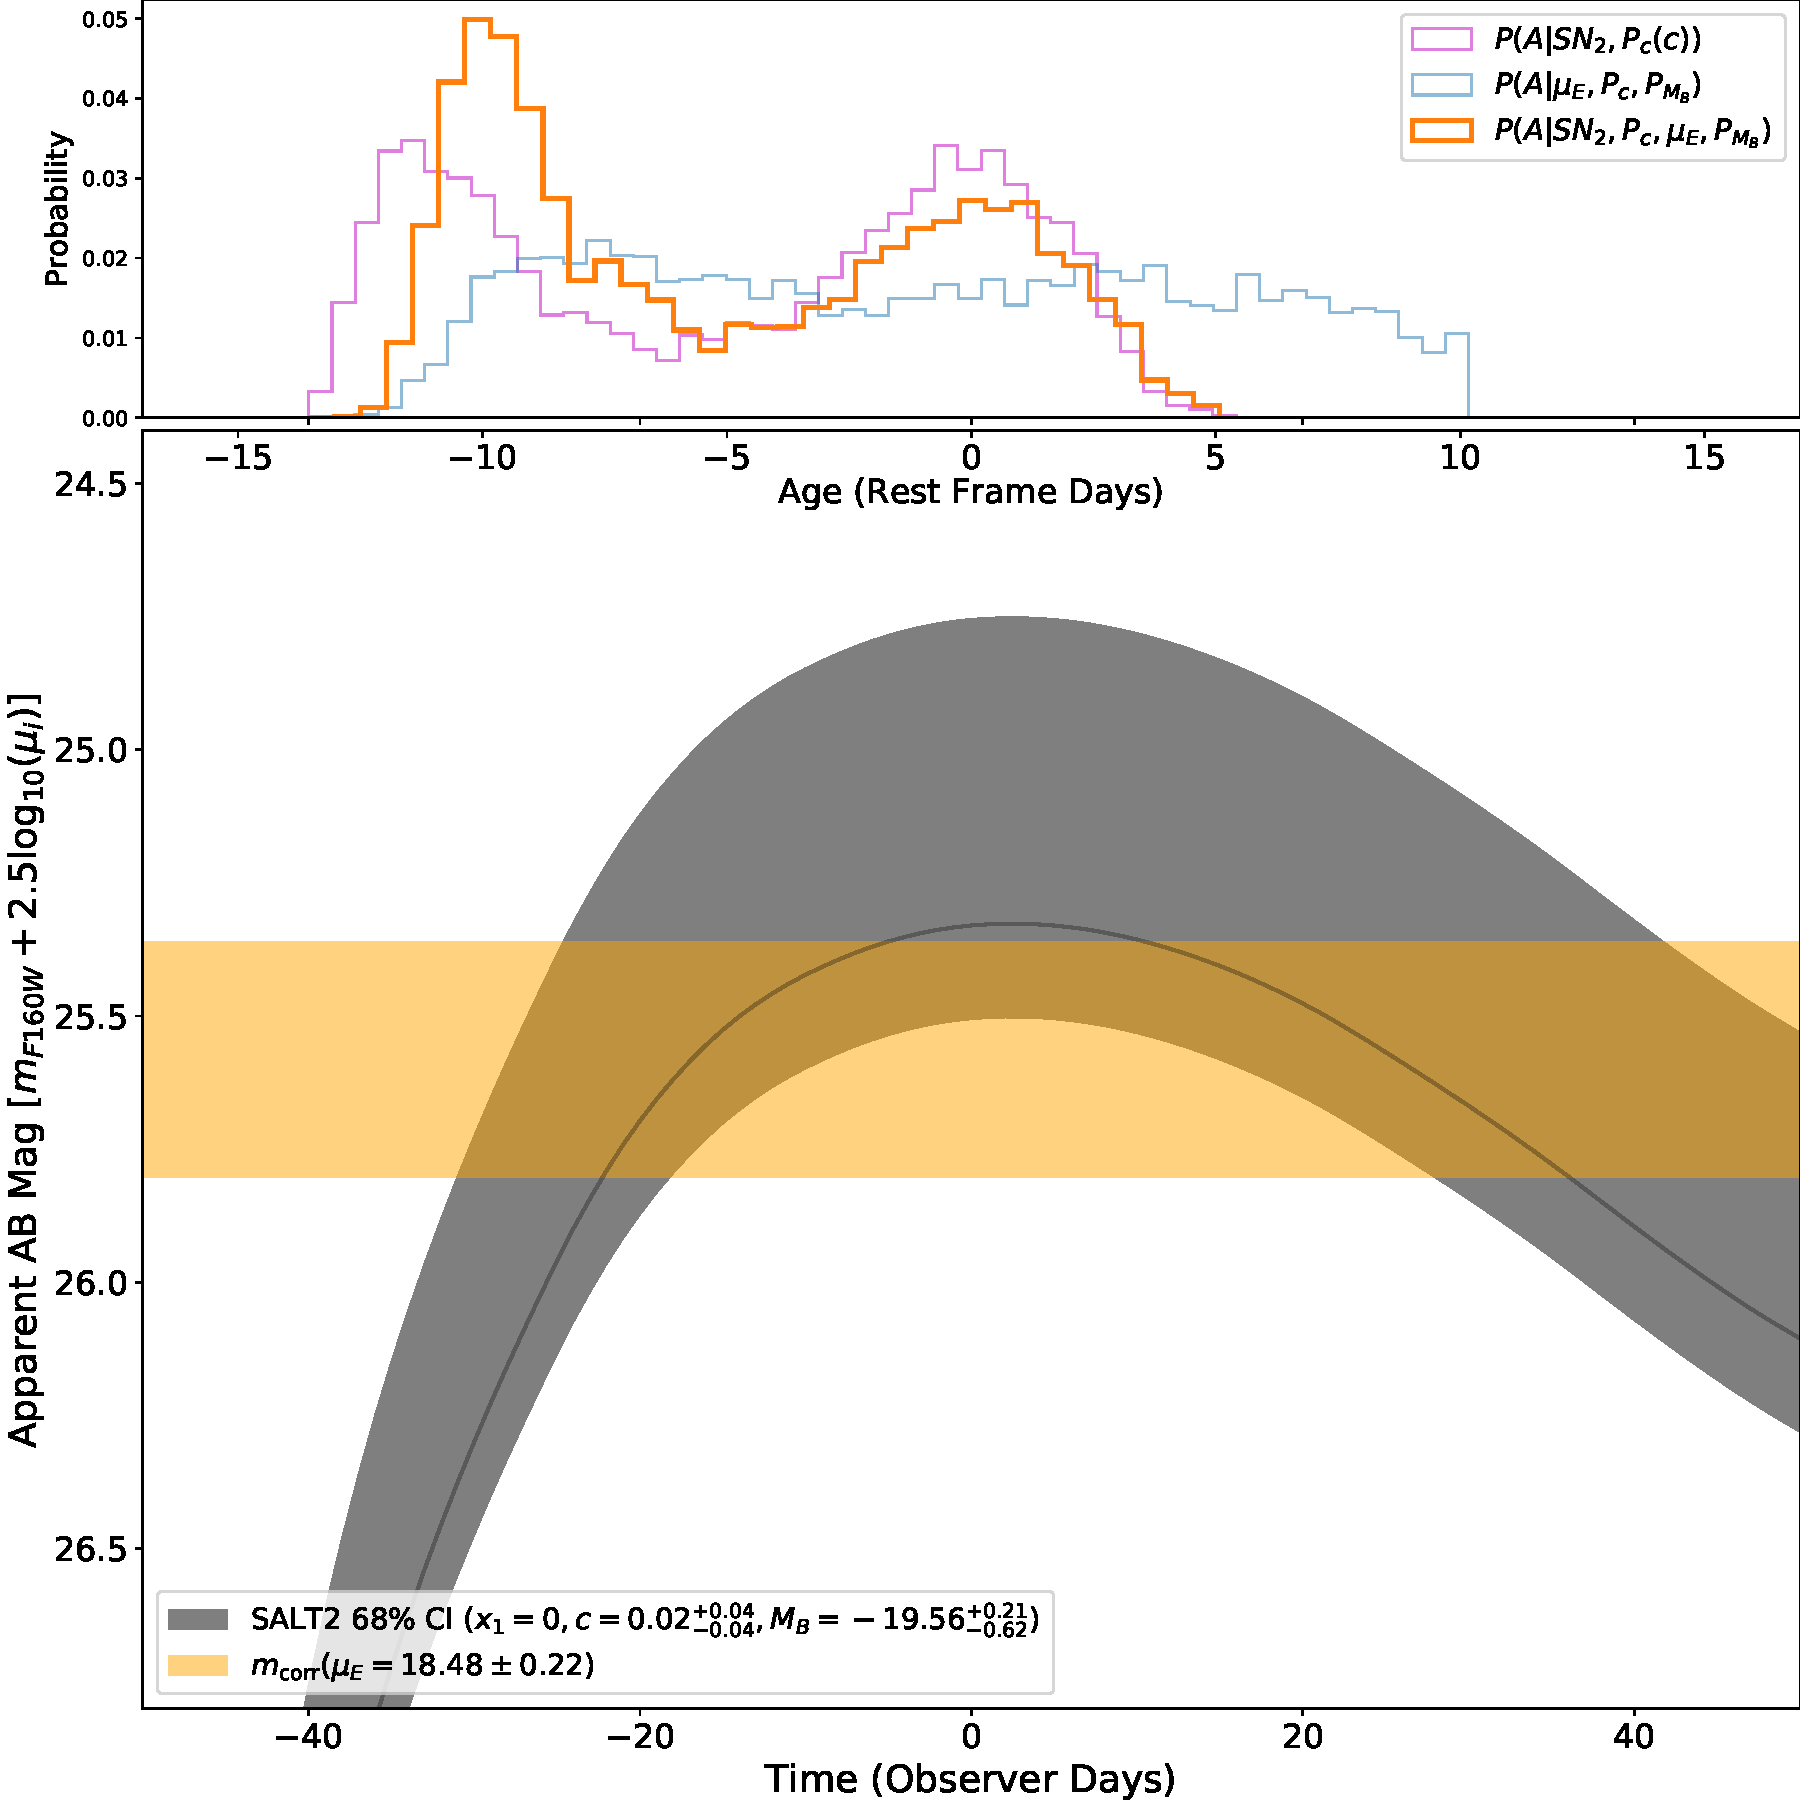
\includegraphics[width=0.45\textwidth]{Images/lightcurve_image2.pdf}
    \caption{Light-curve-based age constraints for \SNABC image 2, using the methodology outlined in section \ref{s:lightcurves}. The upper panel shows the posterior distributions from SNTD for the age of image 2 from section \ref{s:colorcurves} (magenta), section \ref{s:lightcurves} (light blue), and the combination of both methods (orange). The grey shaded region covers the 68\% confidence interval of the best-fit SALT2 light curve, with the median model shown as a solid line. The orange shaded region shows the 1$\sigma$ range of the measured (lens-model-corrected, see table \ref{tab:time_delays}) F160W magnitude, which corresponds to a V band magnitude in the rest-frame. }
    \label{fig:lightcurve2}
\end{figure}

\begin{table}[h]
\begin{tabular}{crrrrrrr}
    
    
    \multicolumn{1}{c}{Model} &\multicolumn{1}{c}{$\mu_1$} & \multicolumn{1}{c}{$\mu_2$} &\multicolumn{1}{c}{$\mu_3$} &\multicolumn{1}{c}{$t_2-t_1$} & \multicolumn{1}{c}{$t_3-t_1$}& \multicolumn{1}{c}{$t_4-t_1$} & \multicolumn{1}{c}{Bayesian Evidence}\\
\midrule
\textit{C} & 6.324 & 9.526 & 6.879 & 180.3 & 82.7&7402.8&$-15.18\pm0.33$ \\
\textit{D} & 6.281 & 9.923 & 7.472 & 184.4 & 85.3&7034.9&$-13.46\pm0.31$ \\
\textit{E} &8.942  & 18.48 & 13.257 & 103.6 & 50.2&5876.8&$-8.91\pm0.27$ \\
\textit{F} & 8.699 & 18.069 & 12.719 & 108.3 & 53.7&6020.5&$-9.67\pm0.28$ \\
\end{tabular}
\caption{\label{tab:model_evidence}Model Preferences}
\end{table}

\subsection*{Final Inferred Time Delays}

As discussed at the end of the previous section, our final age constraints for each SN image are a joint posterior between the parameter estimates from color-curve fitting (lens model independent) and light curve fitting (lens model dependent). We use image 2 as the reference image because of its likely insensitivity to chromatic microlensing,  resulting in the final time delays and uncertainties reported in table \ref{tab:time_delays} of the main text. Using these measured time delays, we can create a reconstructed form of the intrinsic light curve (Fig \ref{fig:full_lightcurve}) and color curve (Fig \ref{fig:full_colorcurve}) of SN Requiem.


The final posterior distribution for image 2 is bi-modal due to a degeneracy that cannot be broken by single epoch photometry, corresponding to a double-peaked intrinsic luminosity posterior for SN Requiem (Fig \ref{fig:corner_combined}). If this degeneracy can be broken with the exquisite photometry expected for the final image of Requiem, then the expected age of image 2 becomes $-31.51^{+2.23}_{-2.01}$, producing a time delay uncertainty for image 4 of $\sim0.04\%$.



\begin{figure*}
    \centering
    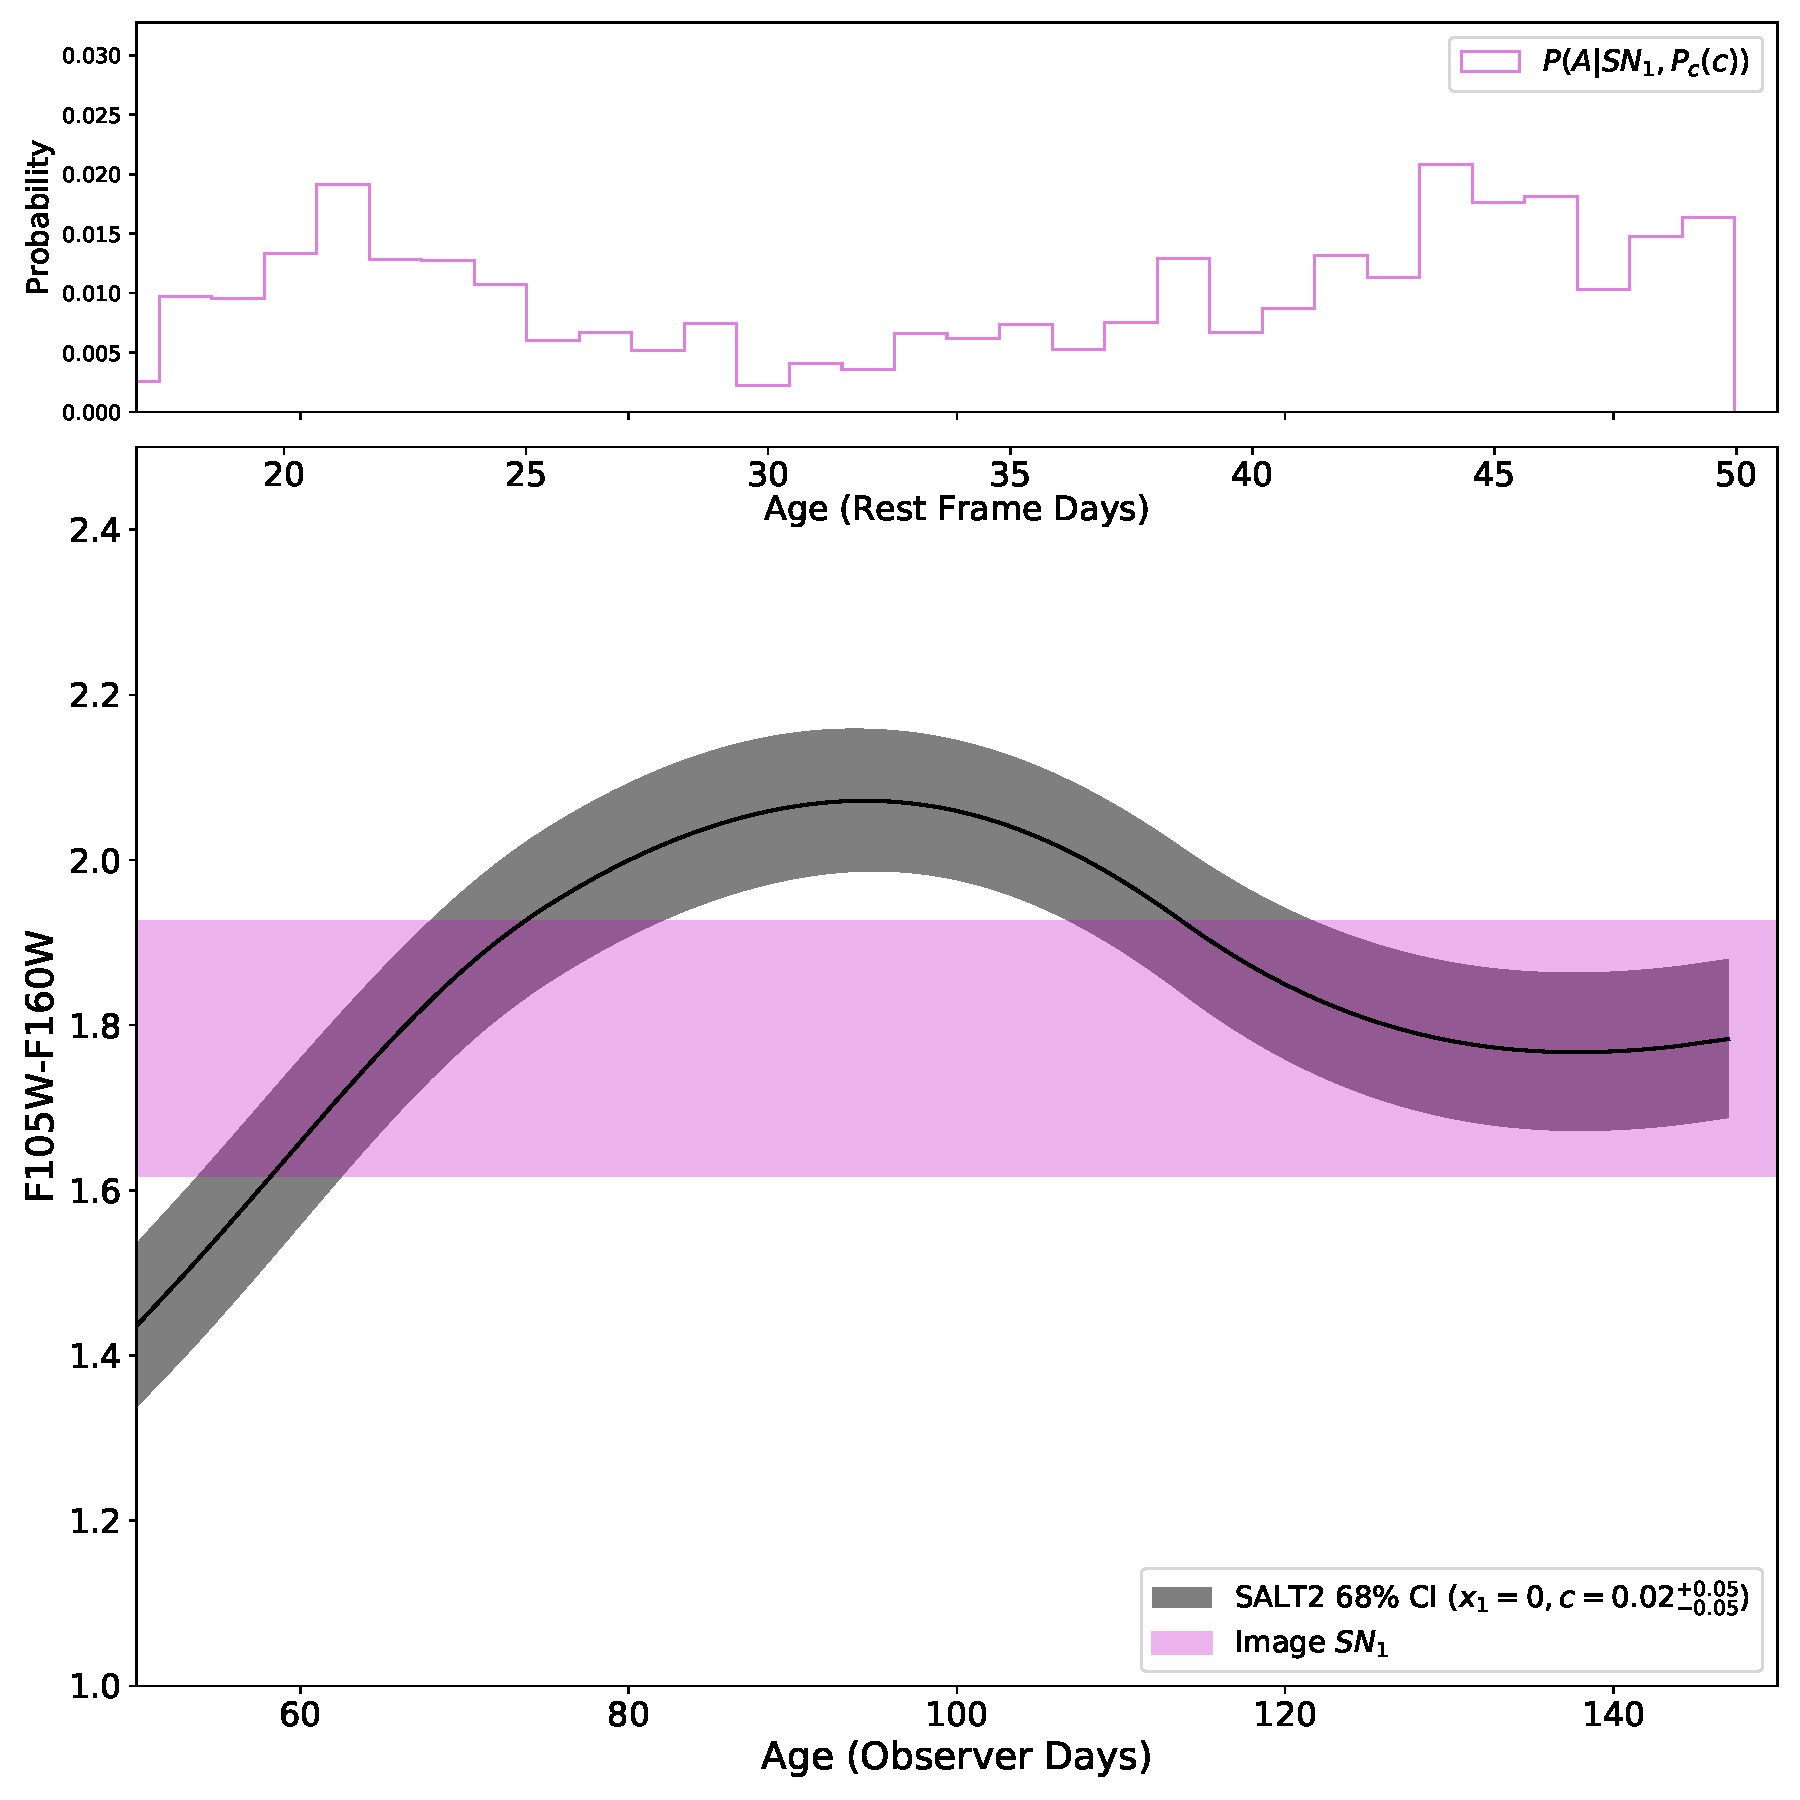
\includegraphics[width=0.45\textwidth]{Images/colorcurve_image1.pdf}
    \caption{Color-based age constraints for \SNABC image 1 and image 3, as in Fig~\ref{fig:colorcurve2}.}
    \label{fig:colorcurve1}
\end{figure*}
\begin{figure*}
    \centering
    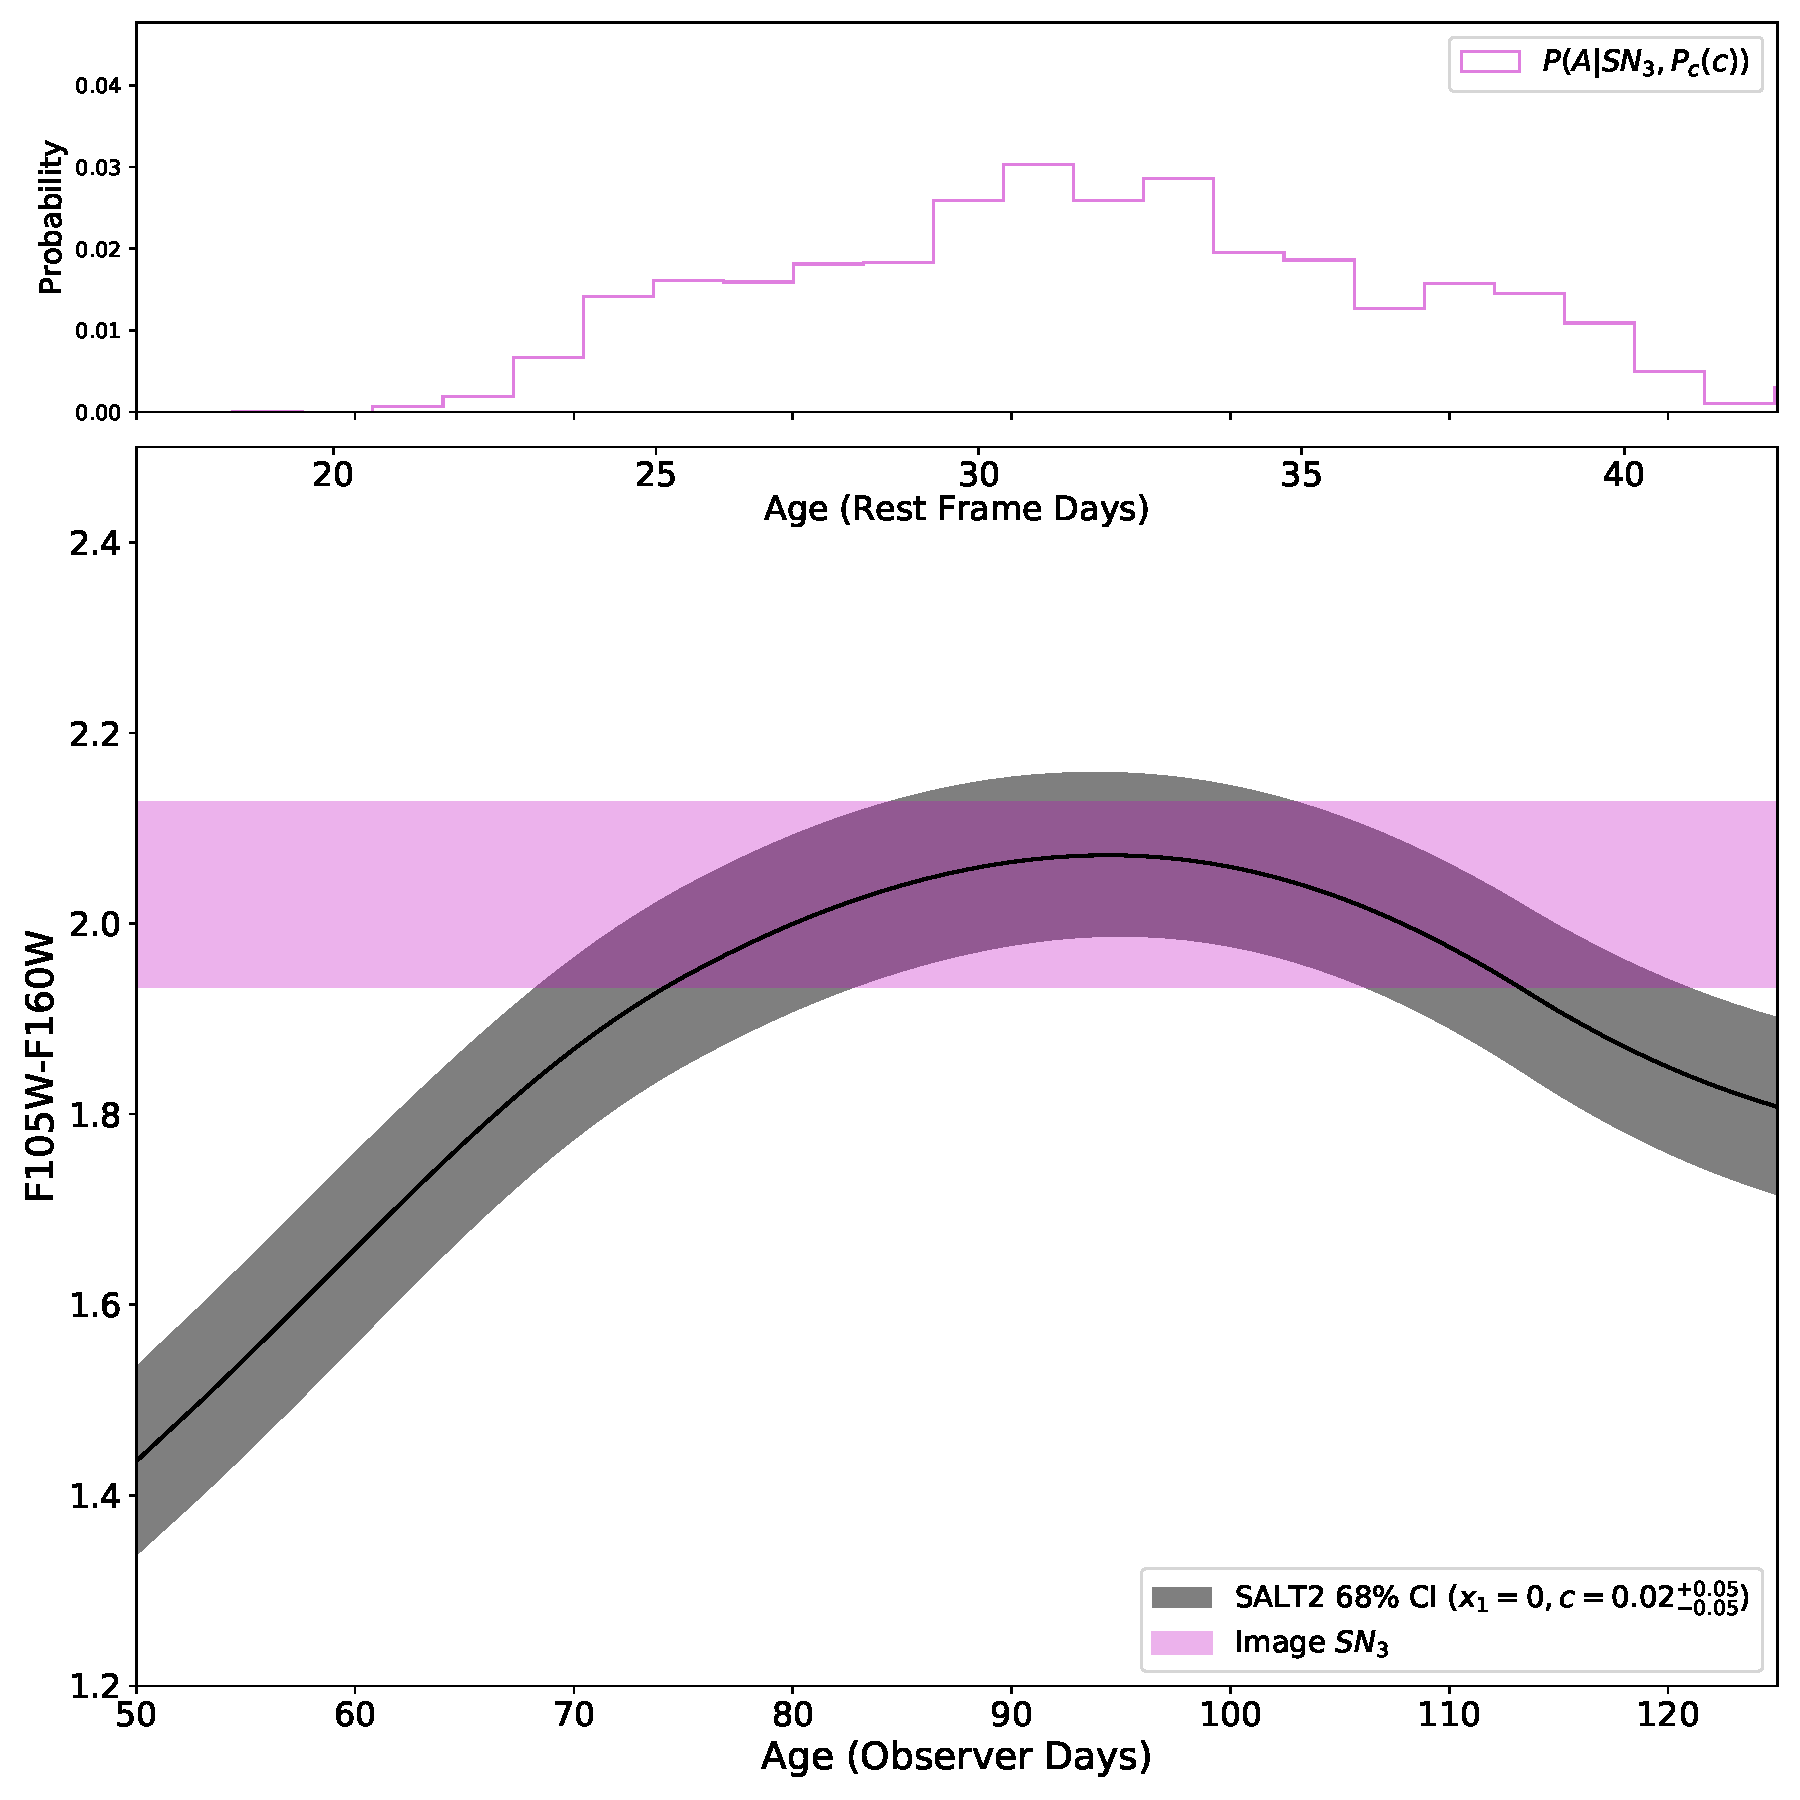
\includegraphics[width=0.45\textwidth]{Images/colorcurve_image3.pdf}
    \caption{Color-based age constraints for \SNABC image 1 and image 3, as in Fig~\ref{fig:colorcurve2}.}
    \label{fig:colorcurve3}
\end{figure*}


\begin{figure*}
    \centering
    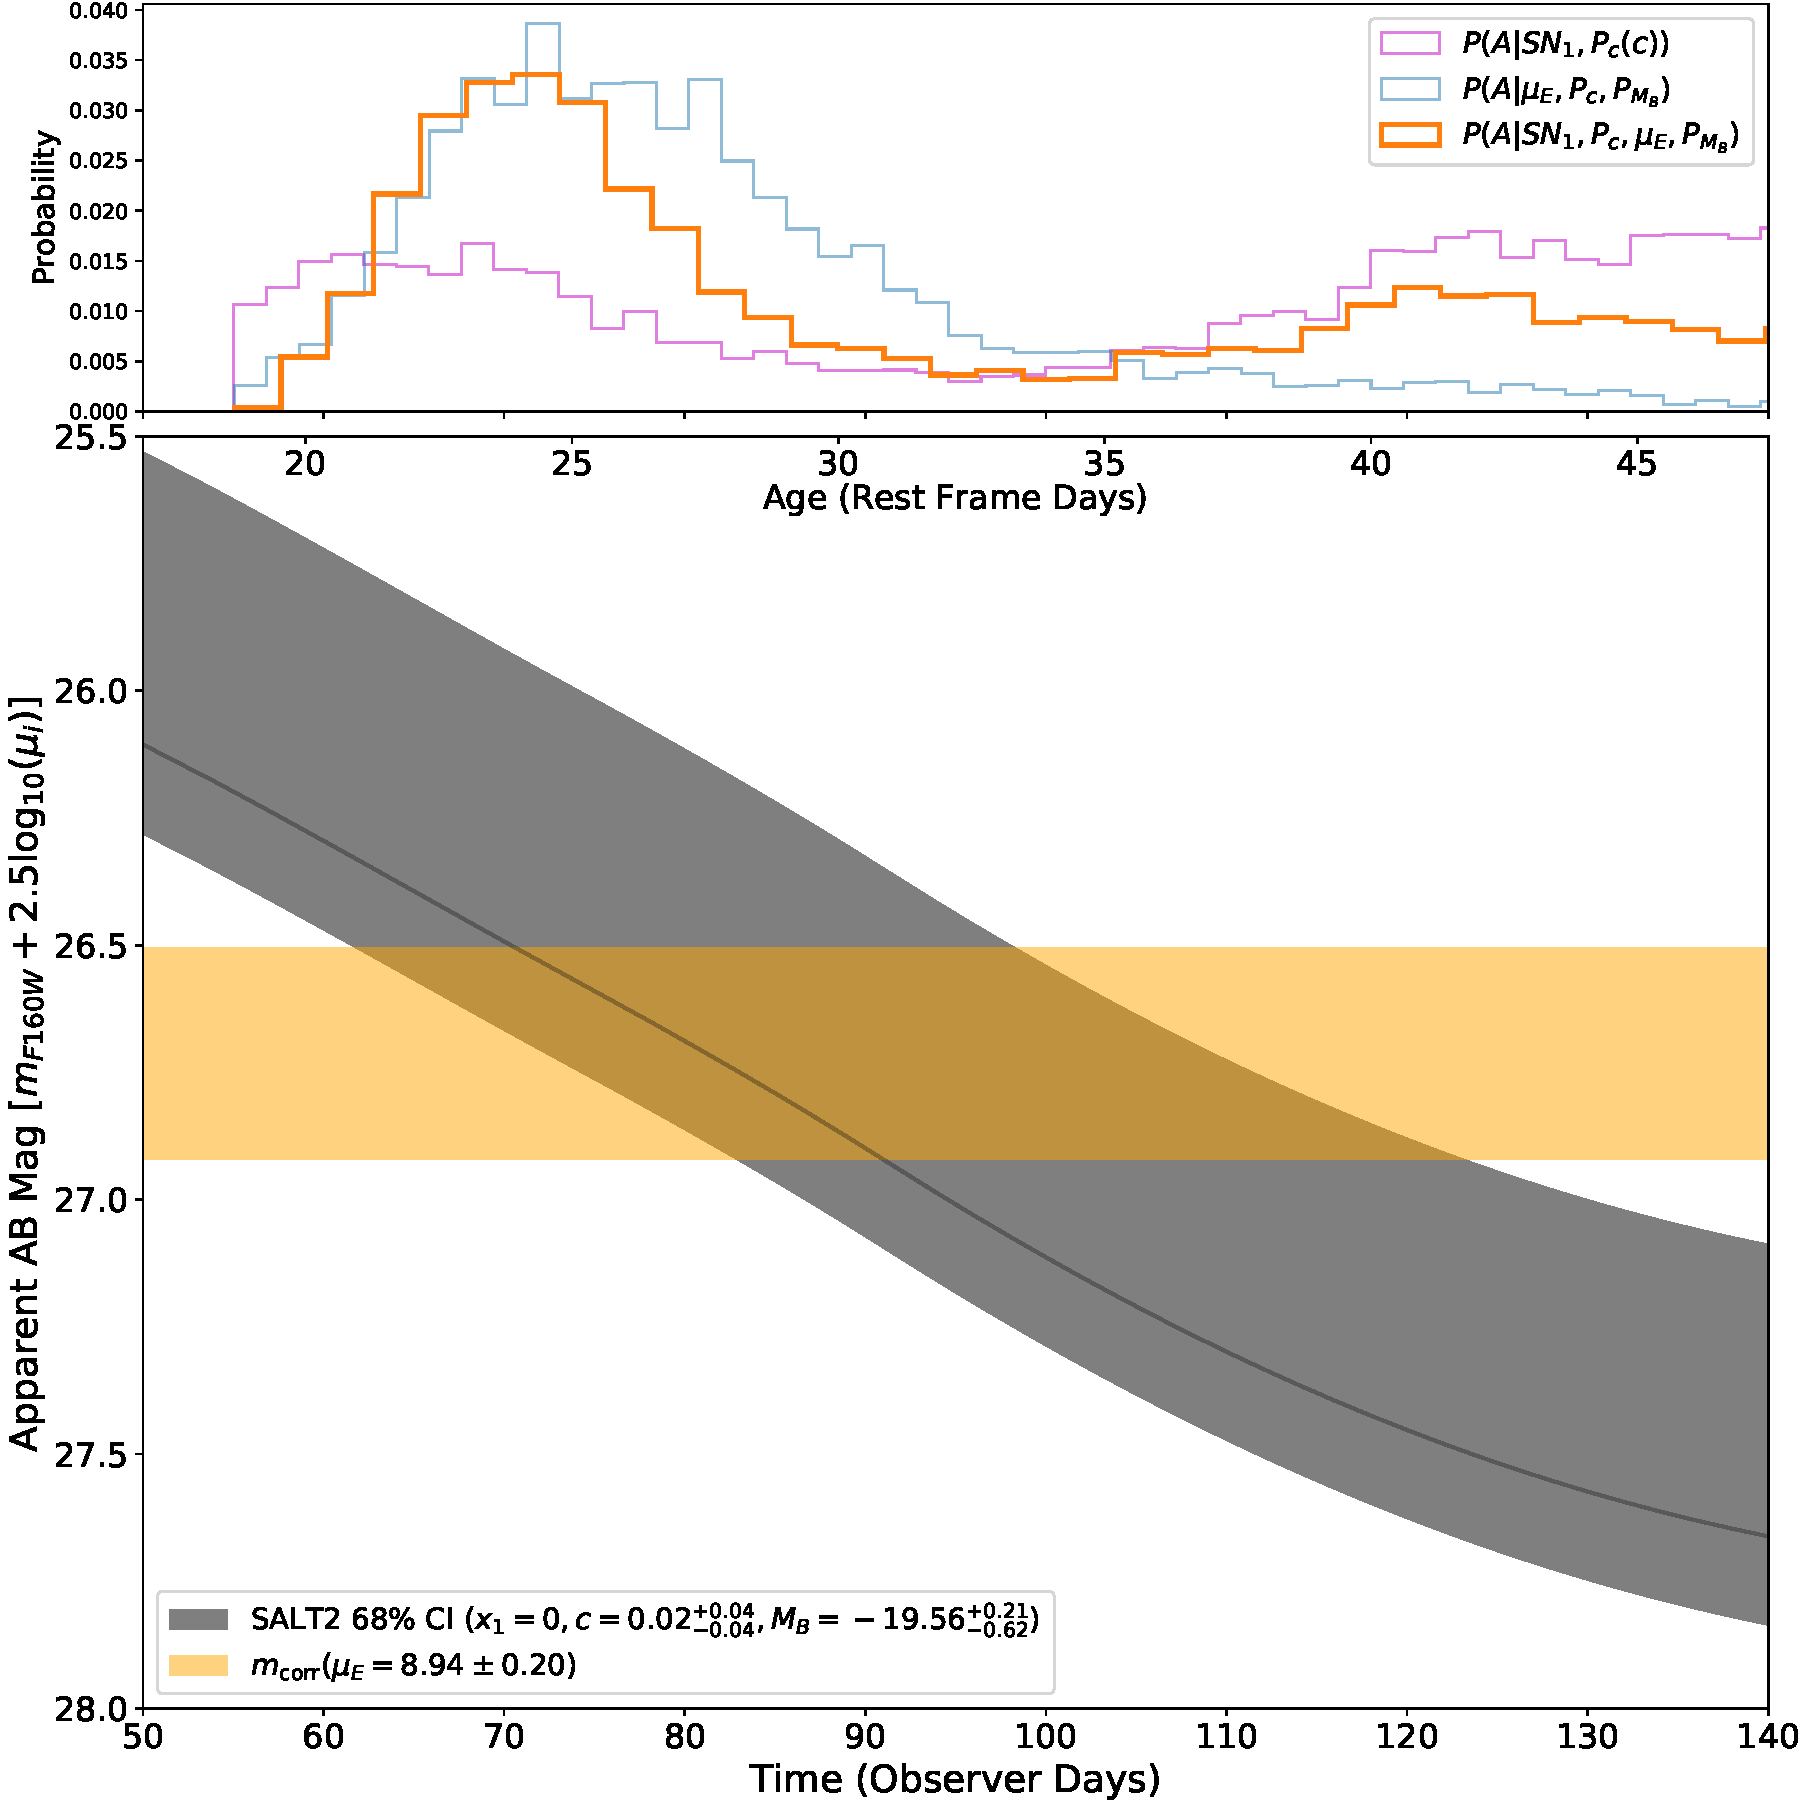
\includegraphics[width=0.45\textwidth]{Images/lightcurve_image1.pdf}
    \caption{Light-curve-based age constraints for \SNABC images 1 and 3.}
    \label{fig:lightcurve1}
\end{figure*}
\begin{figure*}
    \centering
    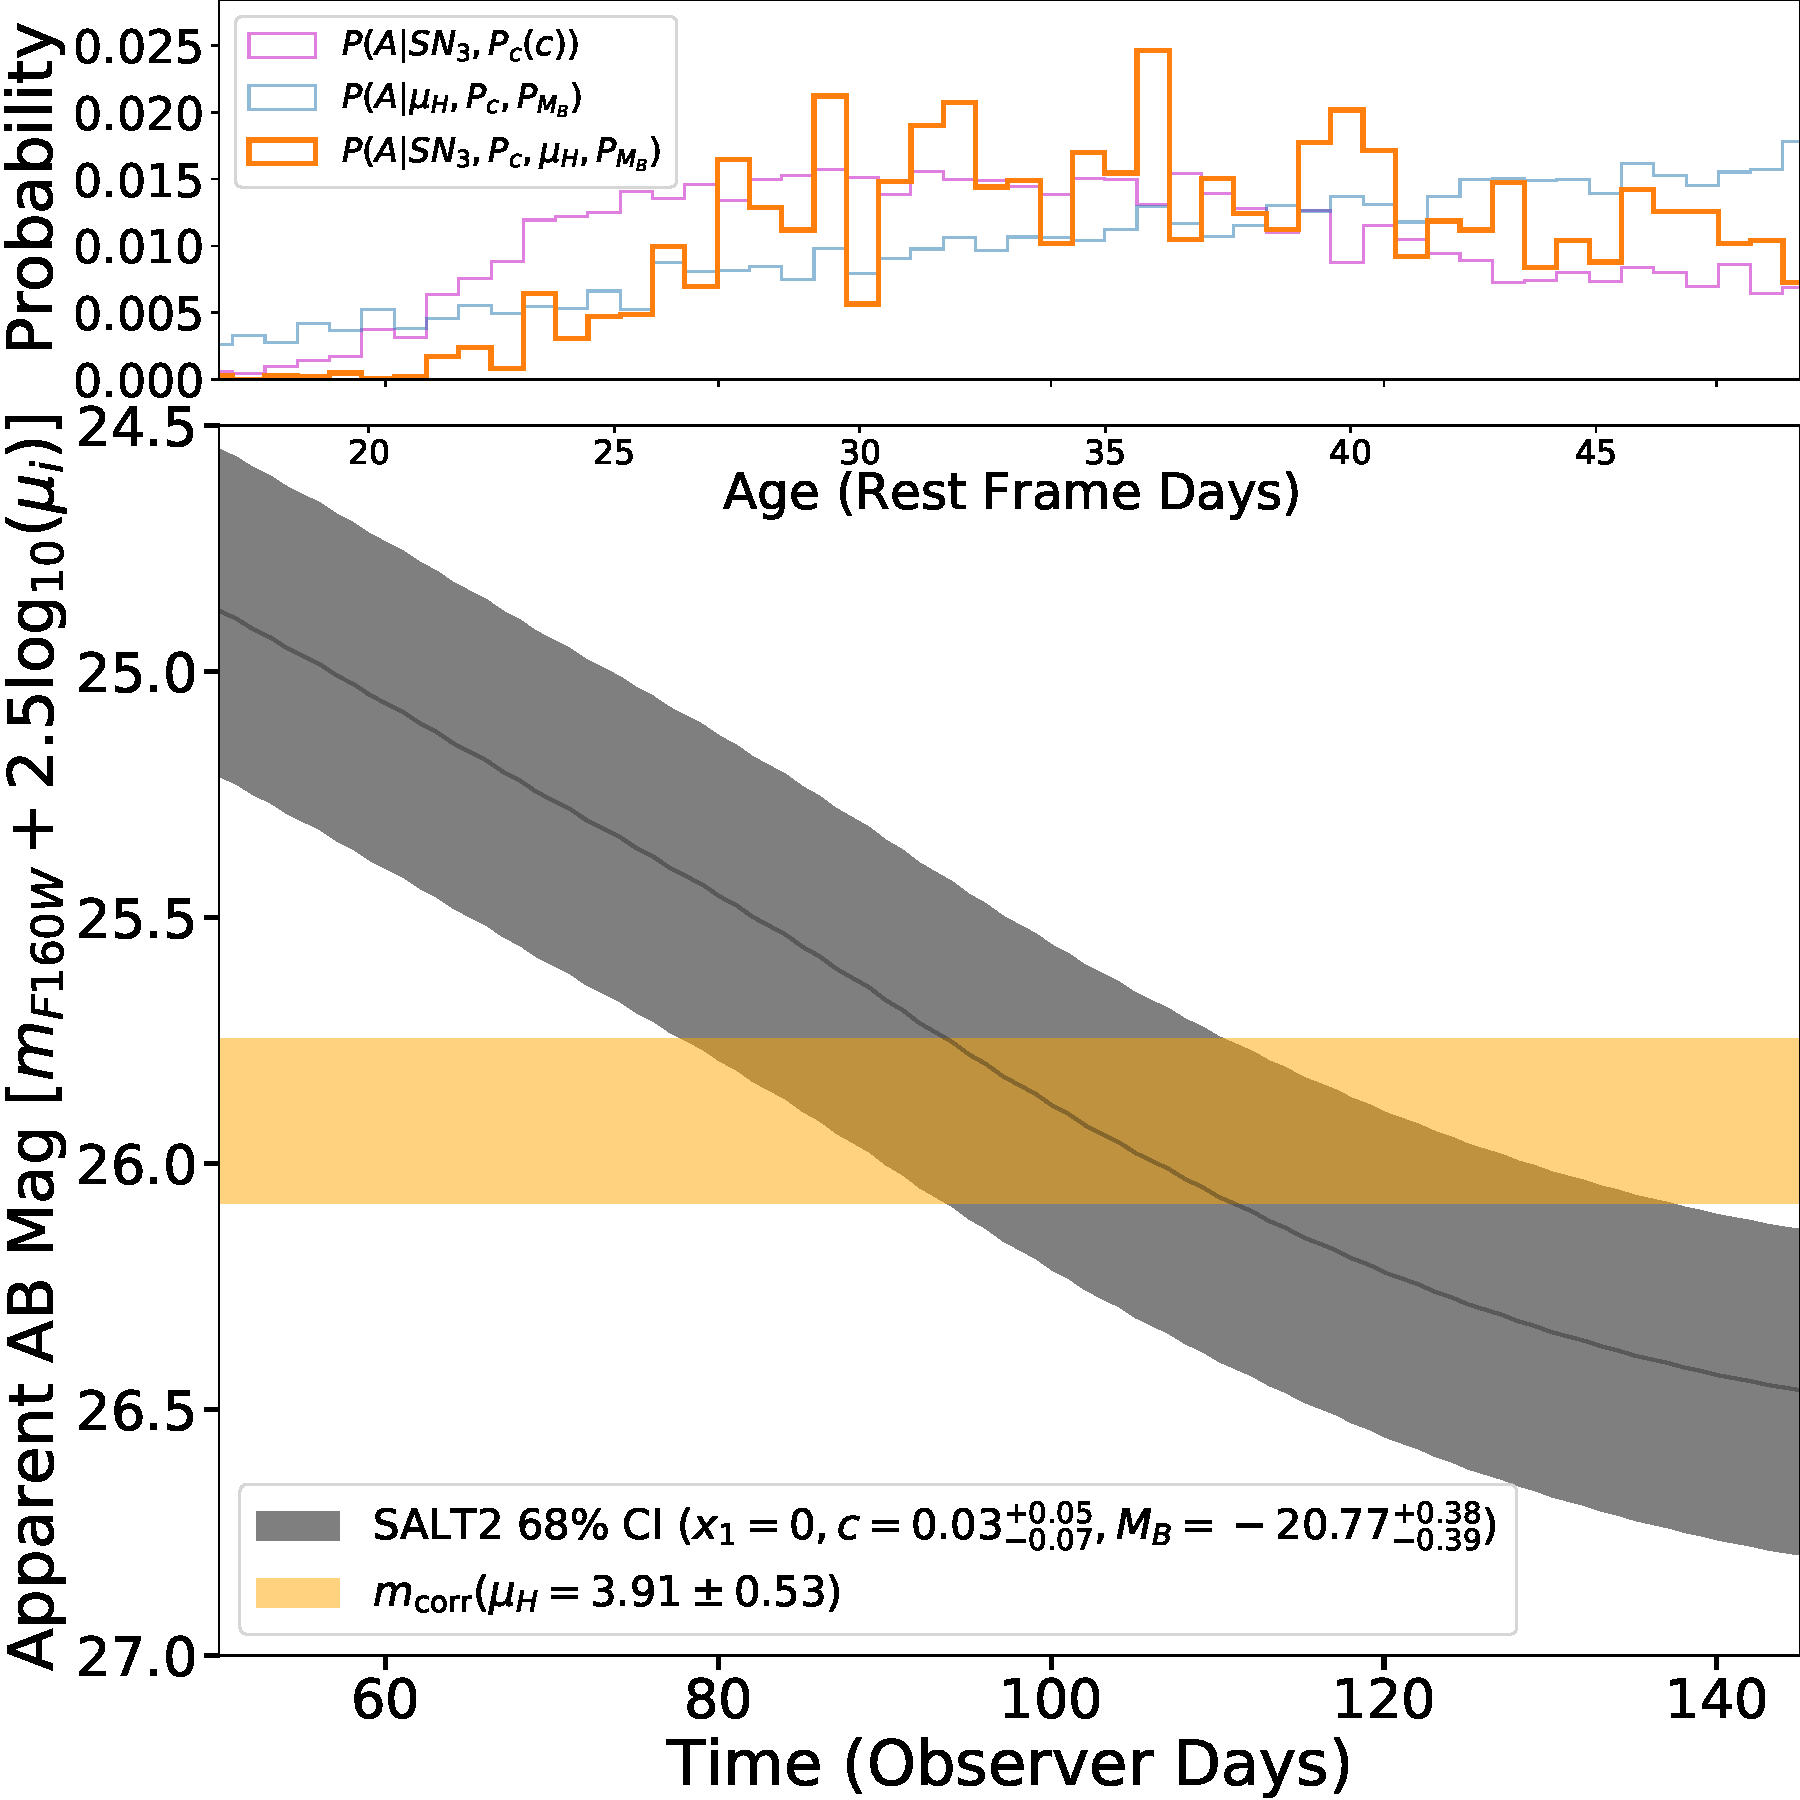
\includegraphics[width=0.45\textwidth]{Images/lightcurve_image3.pdf}
    \caption{Light-curve-based age constraints for \SNABC images 1 and 3.}
    \label{fig:lightcurve3}
\end{figure*}

\begin{figure*}
    \centering
    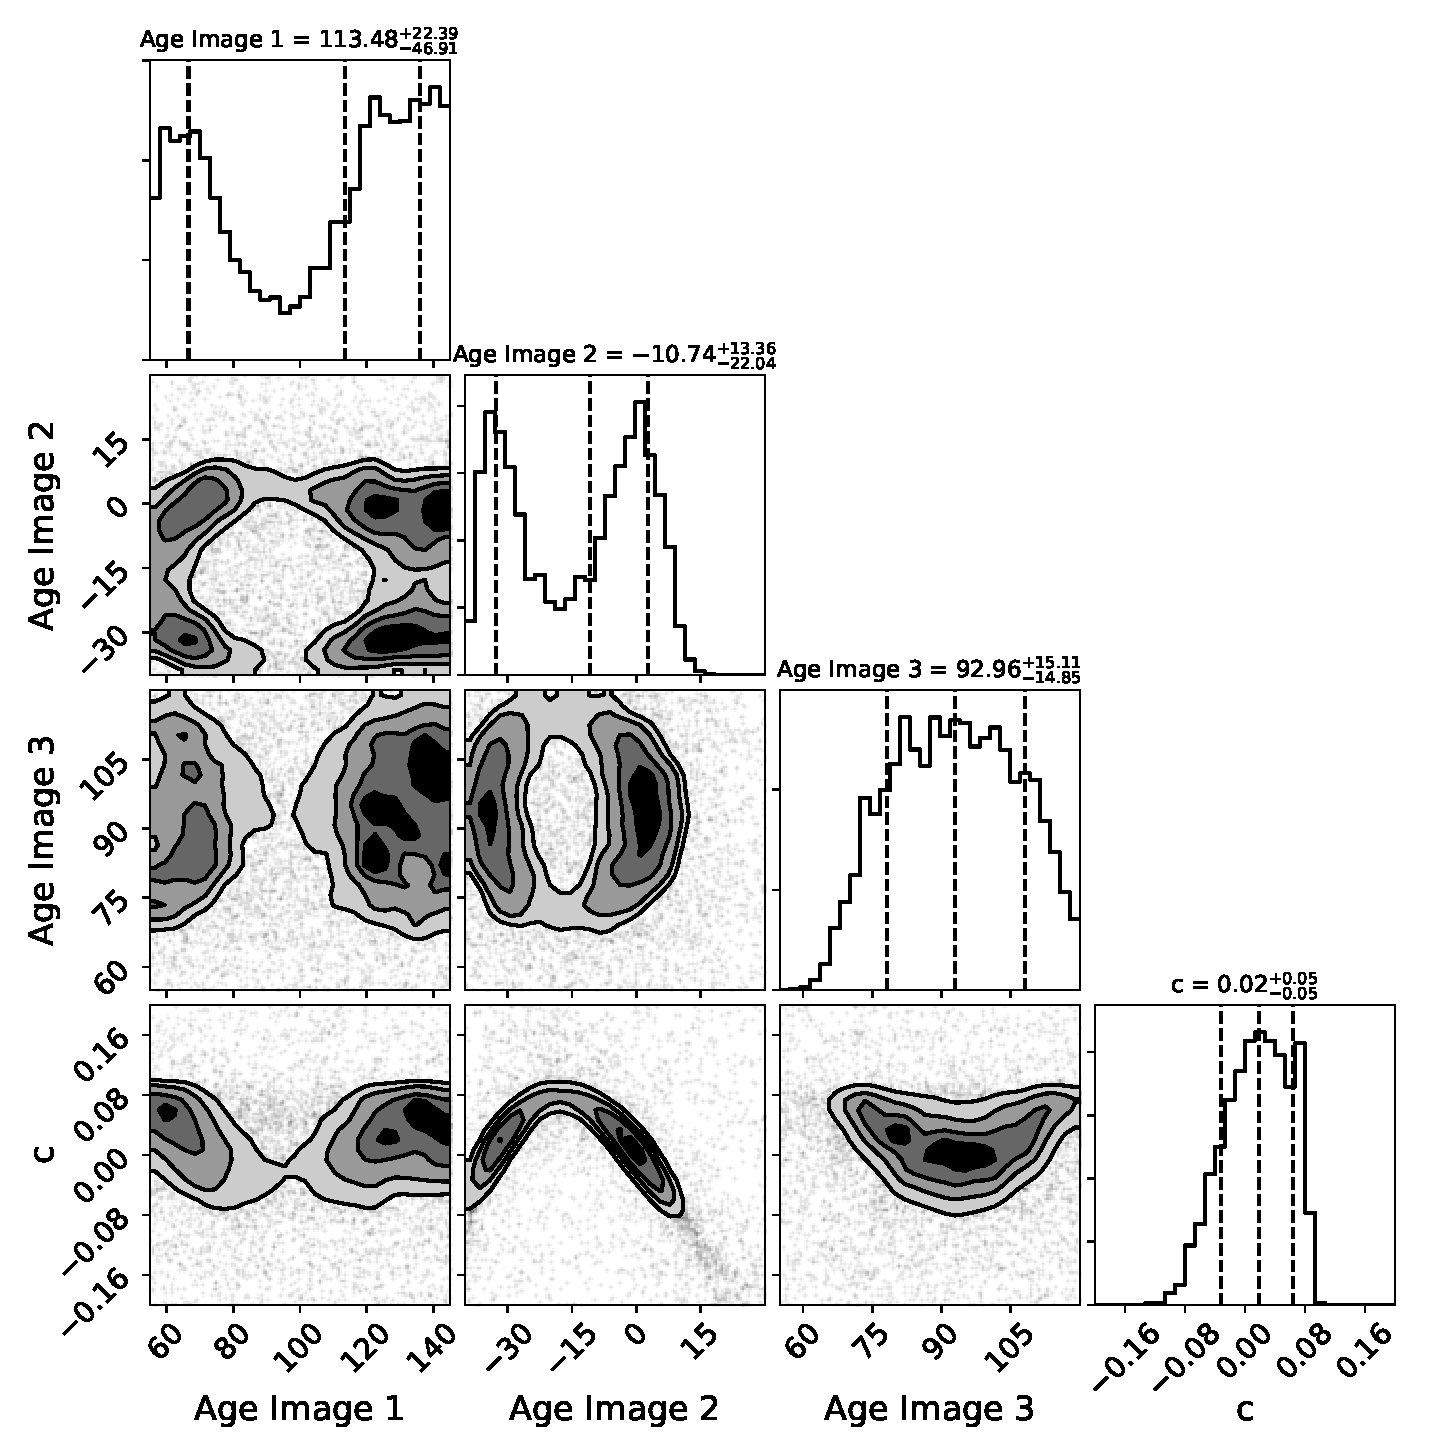
\includegraphics[width=0.75\textwidth]{Images/corner_color_curve_fit_with_c_prior.pdf}
    \caption{Corner plot for color curve nested sampling with prior on c.}
    \label{fig:corner_cfit}
\end{figure*}
\begin{figure*}
    \centering
    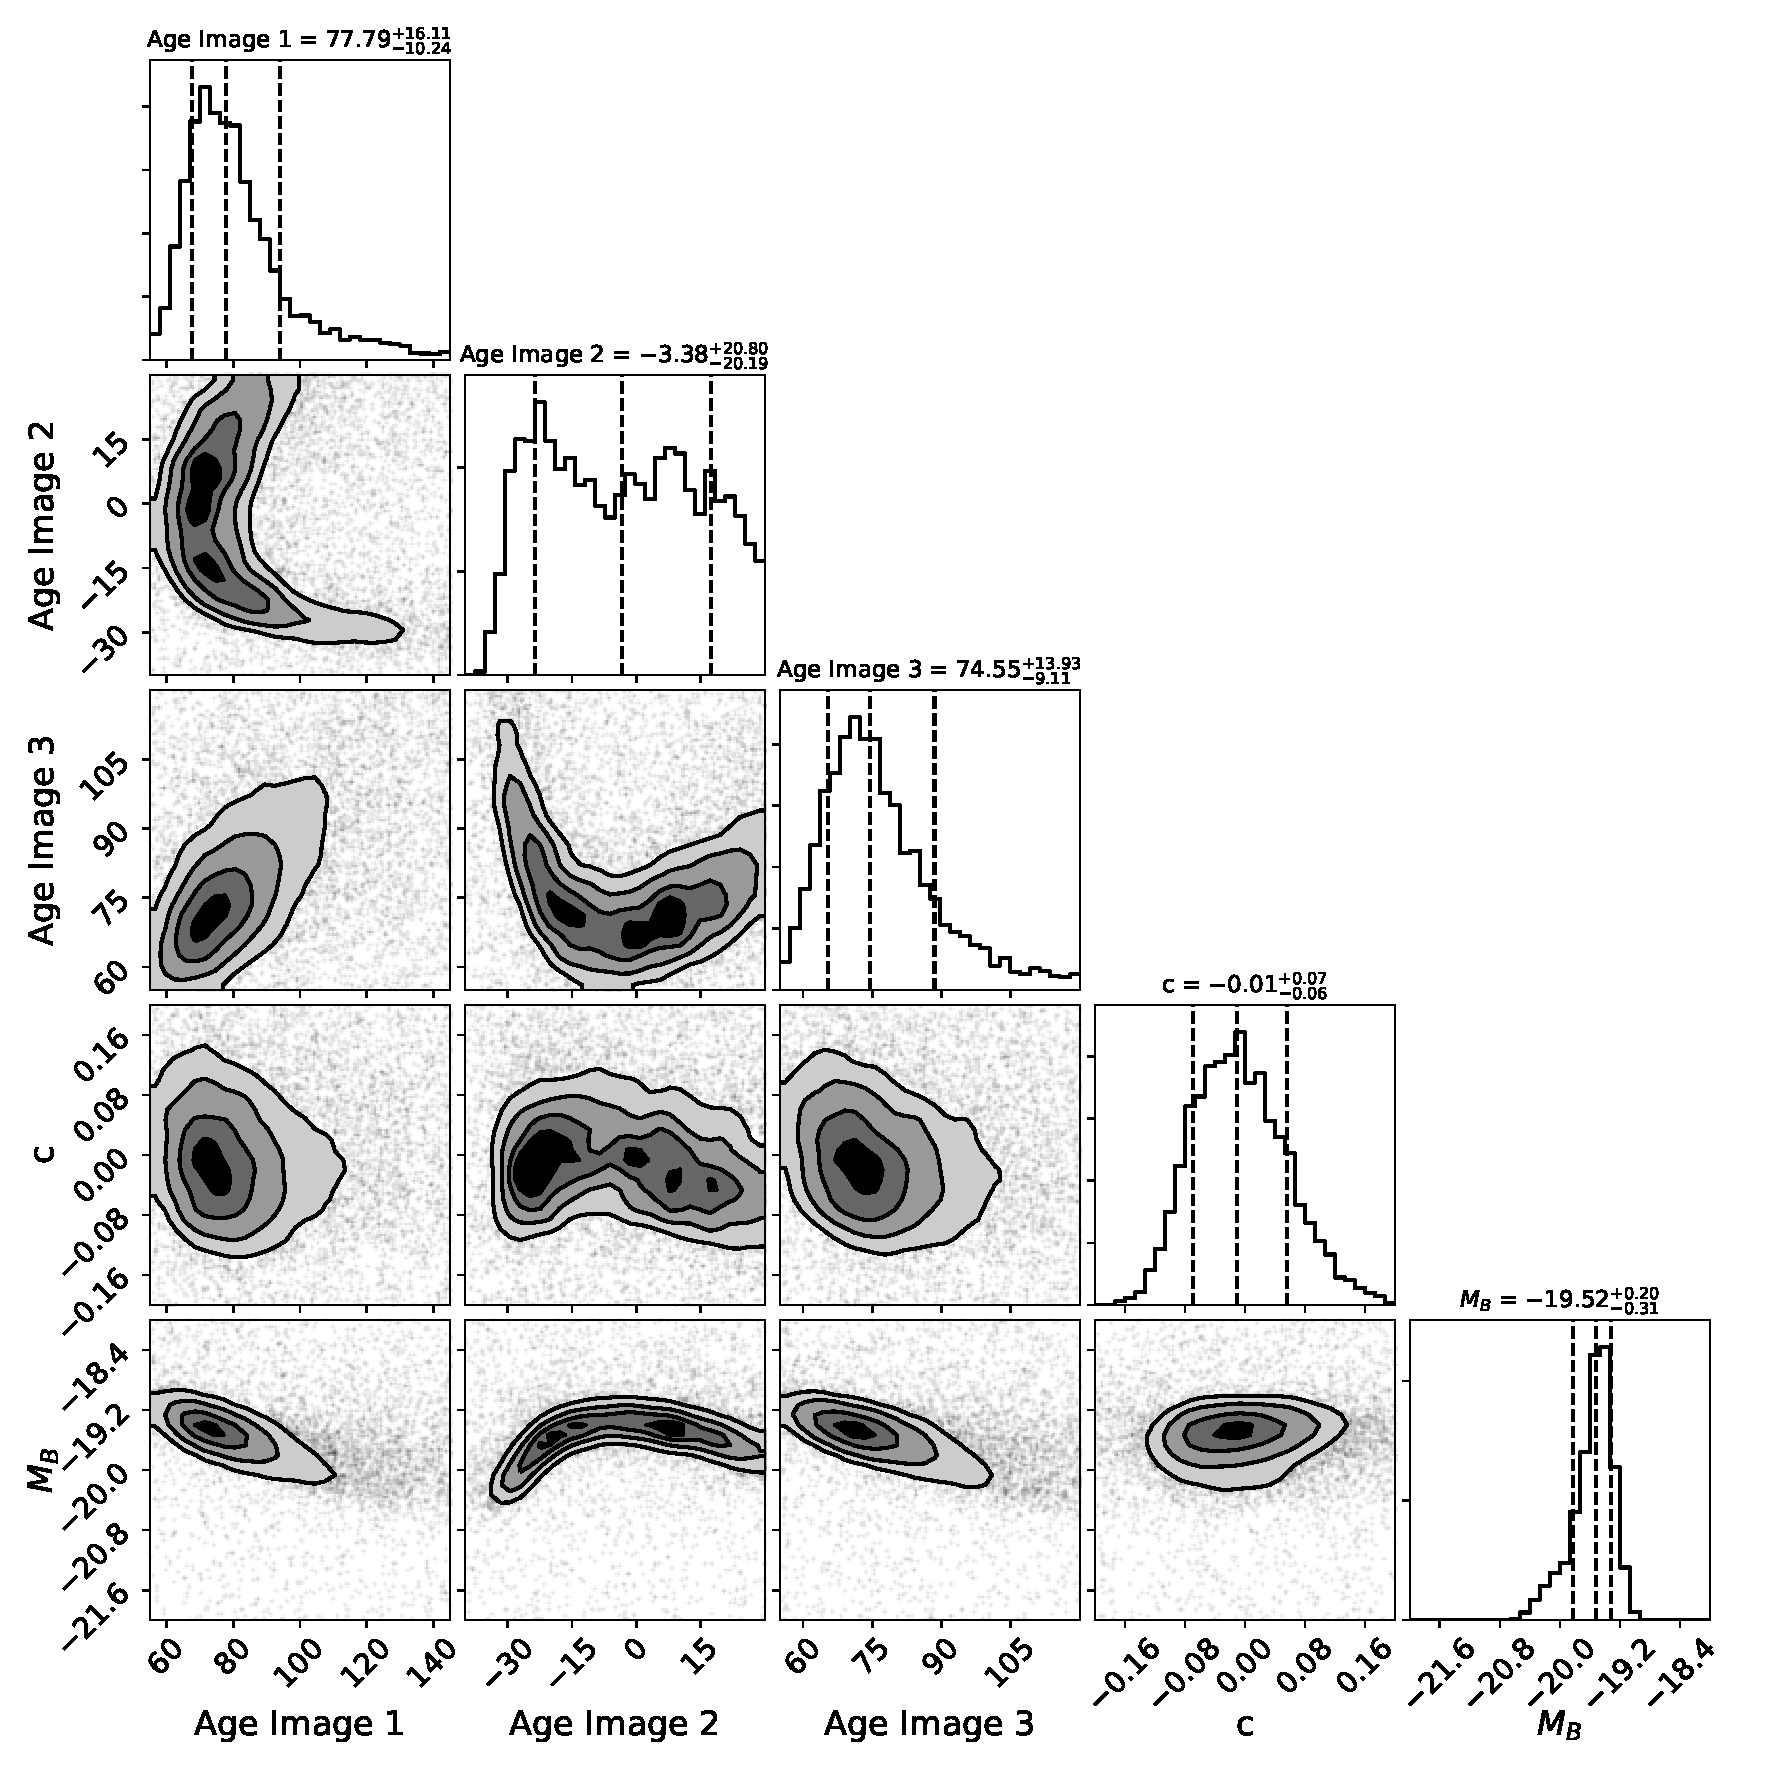
\includegraphics[width=0.75\textwidth]{Images/corner_model_E.pdf}
    \caption{Corner plot for light curve nested sampling using model E.}
    \label{fig:corner_modelE}
\end{figure*}
\begin{figure*}
    \centering
    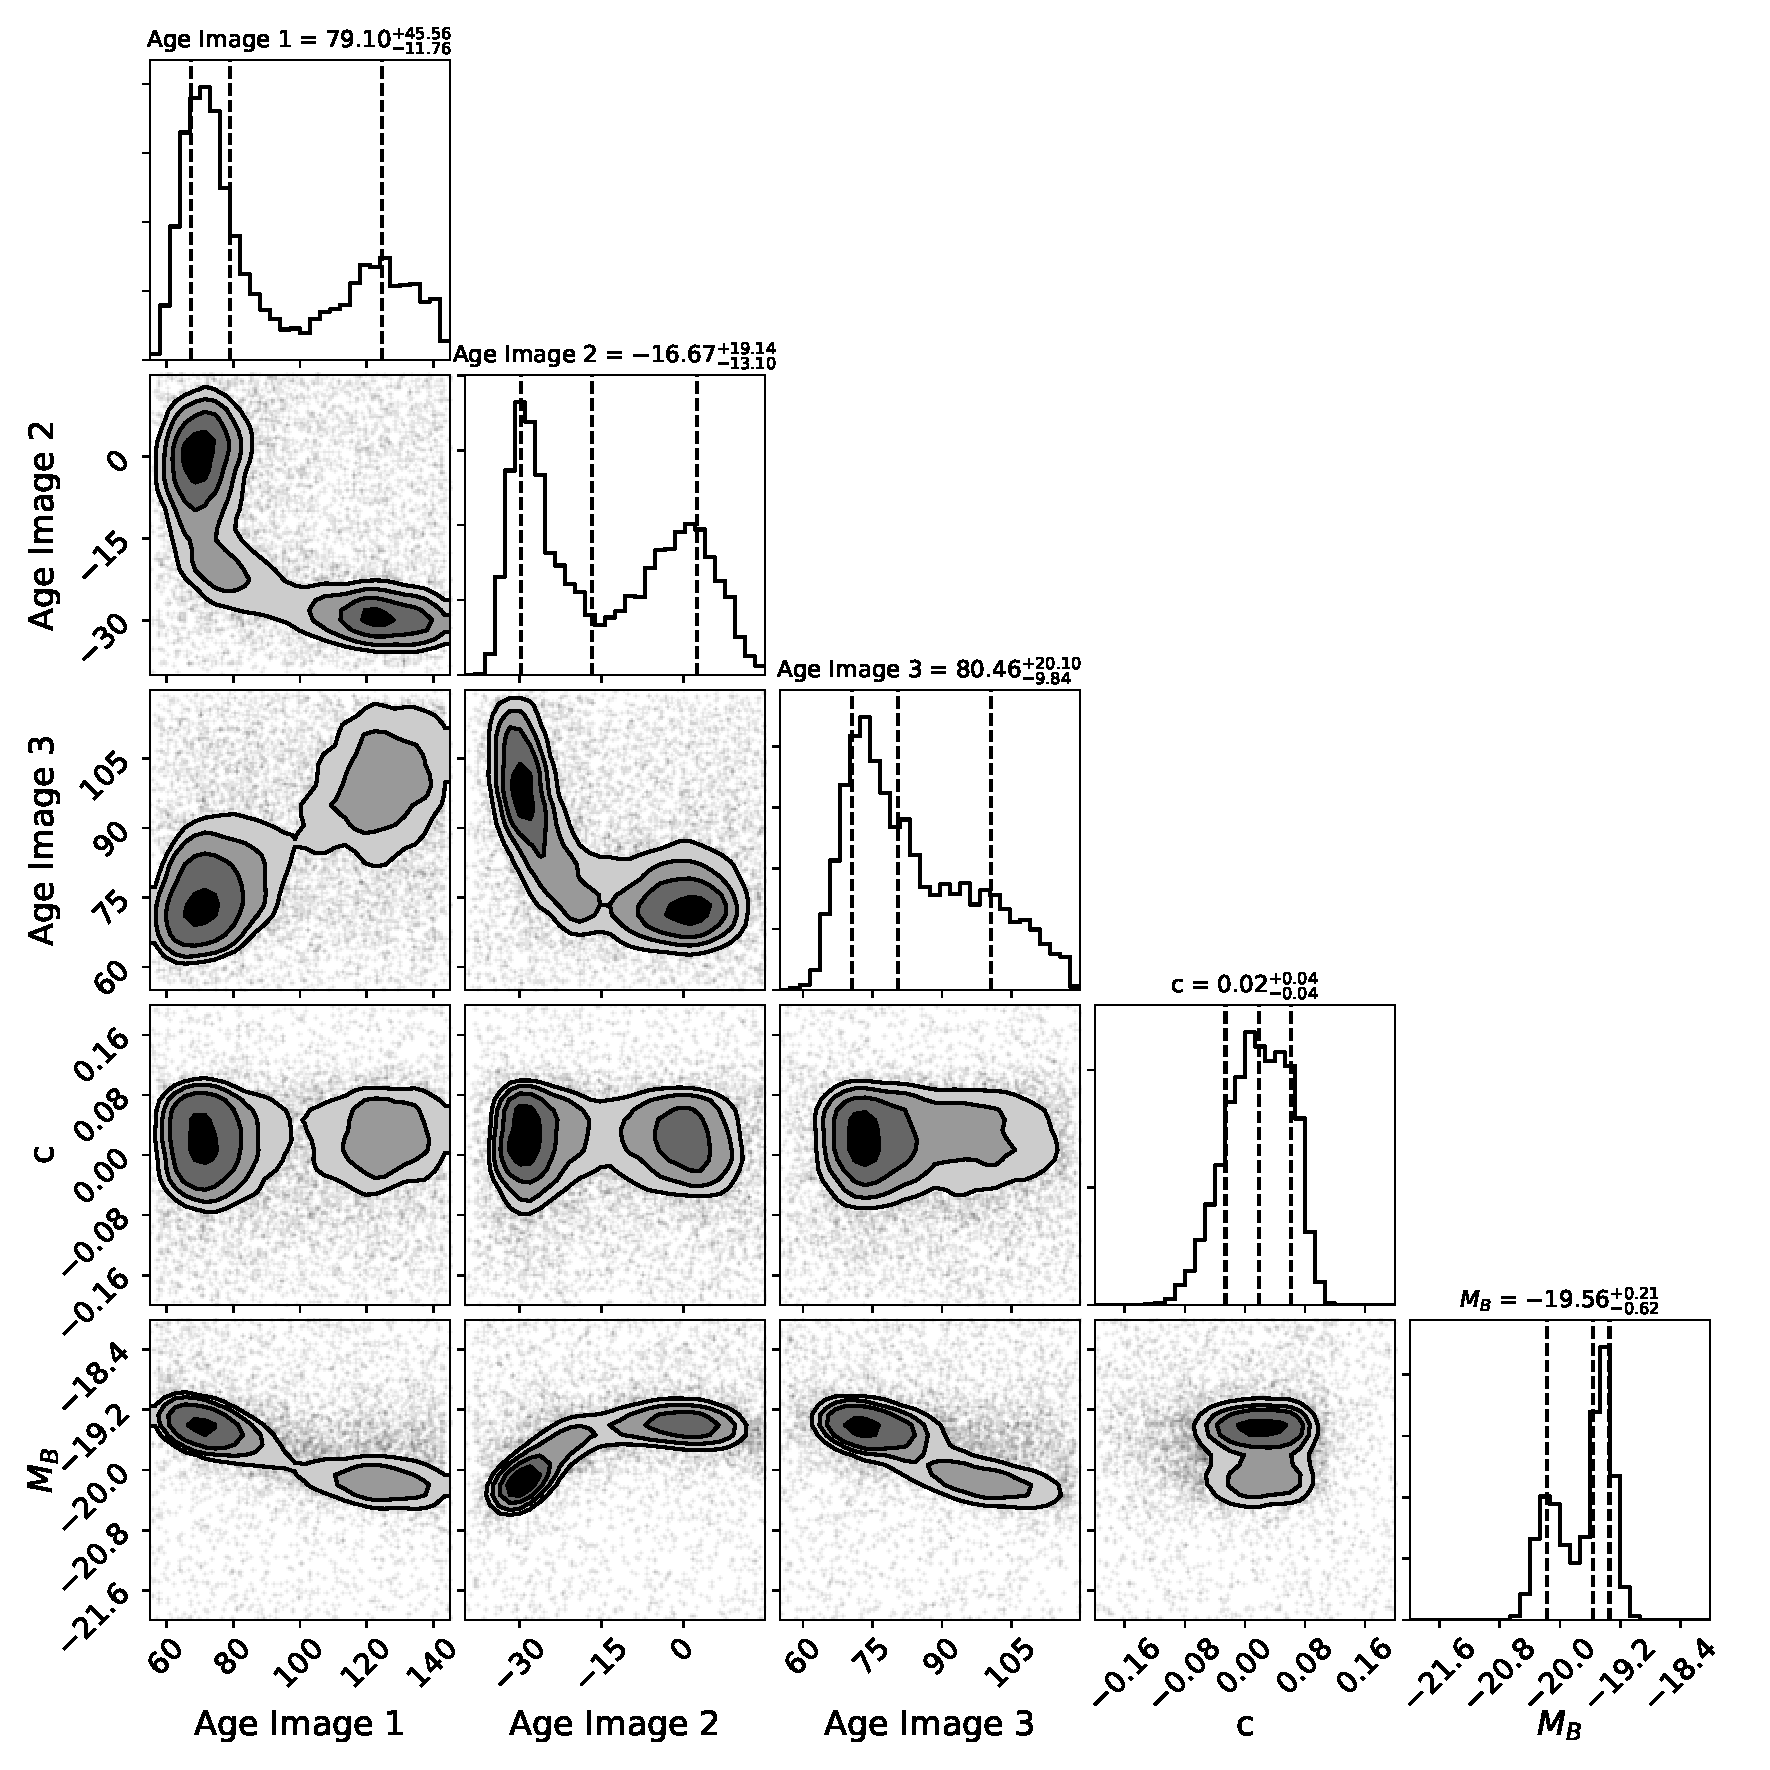
\includegraphics[width=0.75\textwidth]{Images/corner_combined_lc_color_model_E.pdf}
    \caption{Corner plot for combined color curve and model E light curve nested sampling.}
    \label{fig:corner_combined}
\end{figure*}

\begin{figure}[h!]
    \centering
    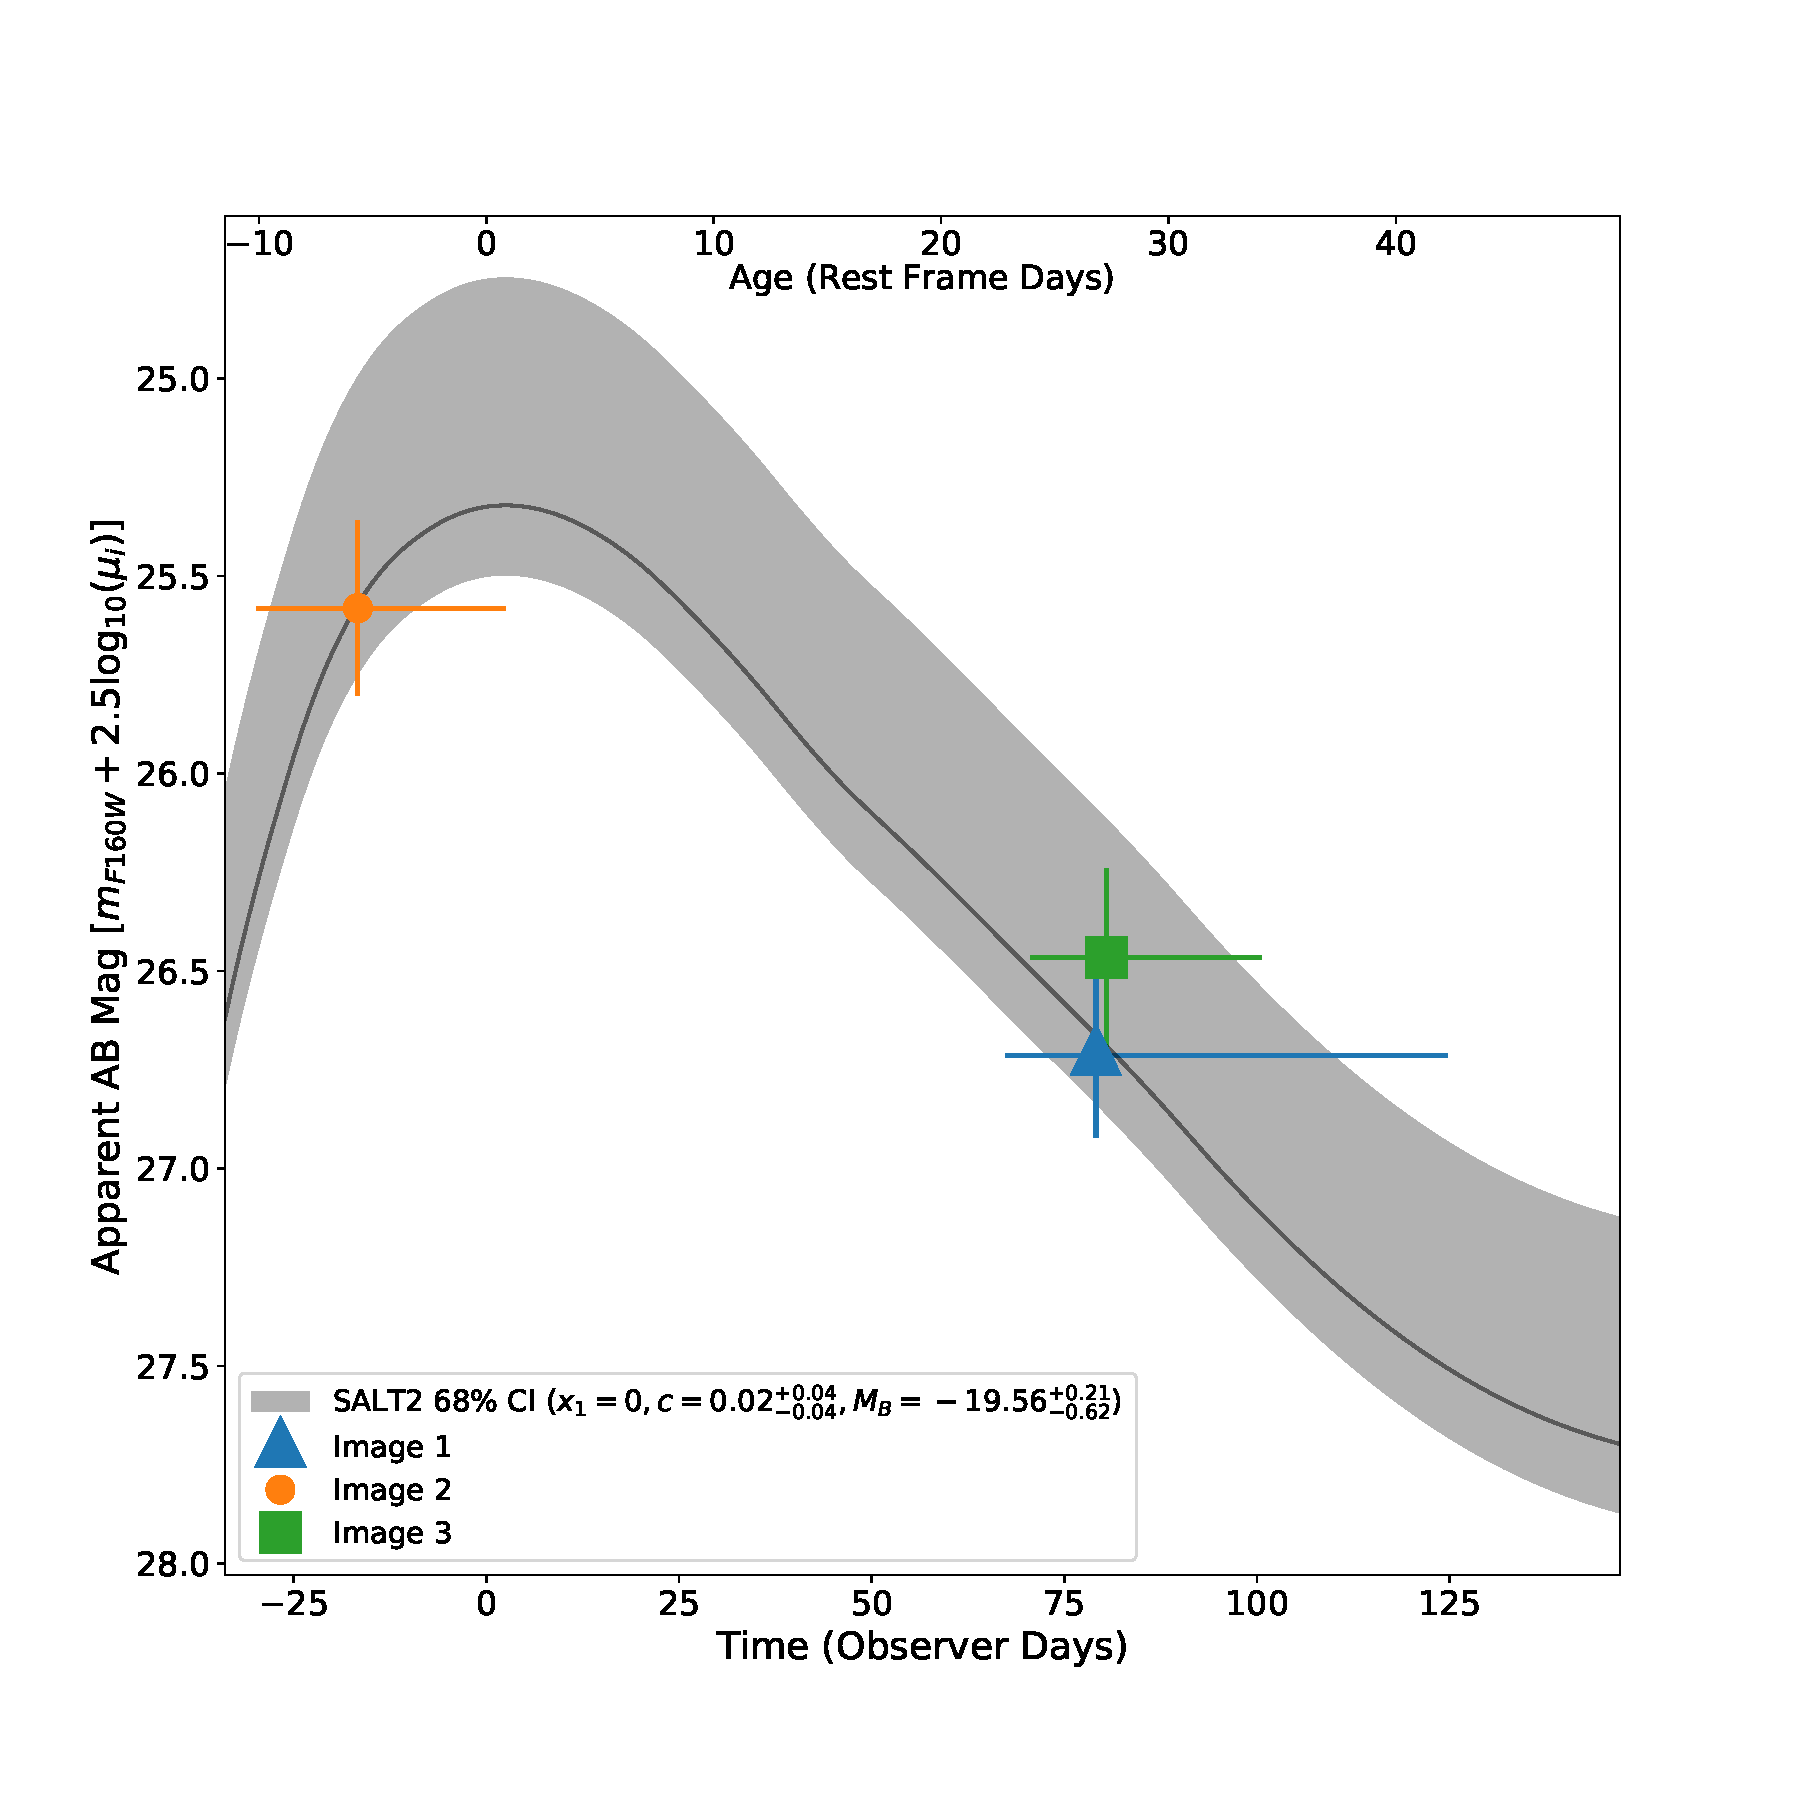
\includegraphics[width=\textwidth]{Paper/Figures/full_lightcurve_full.pdf}
    \caption{\label{fig:full_lightcurve}}
\end{figure}
\begin{figure}[h!]
    \centering
    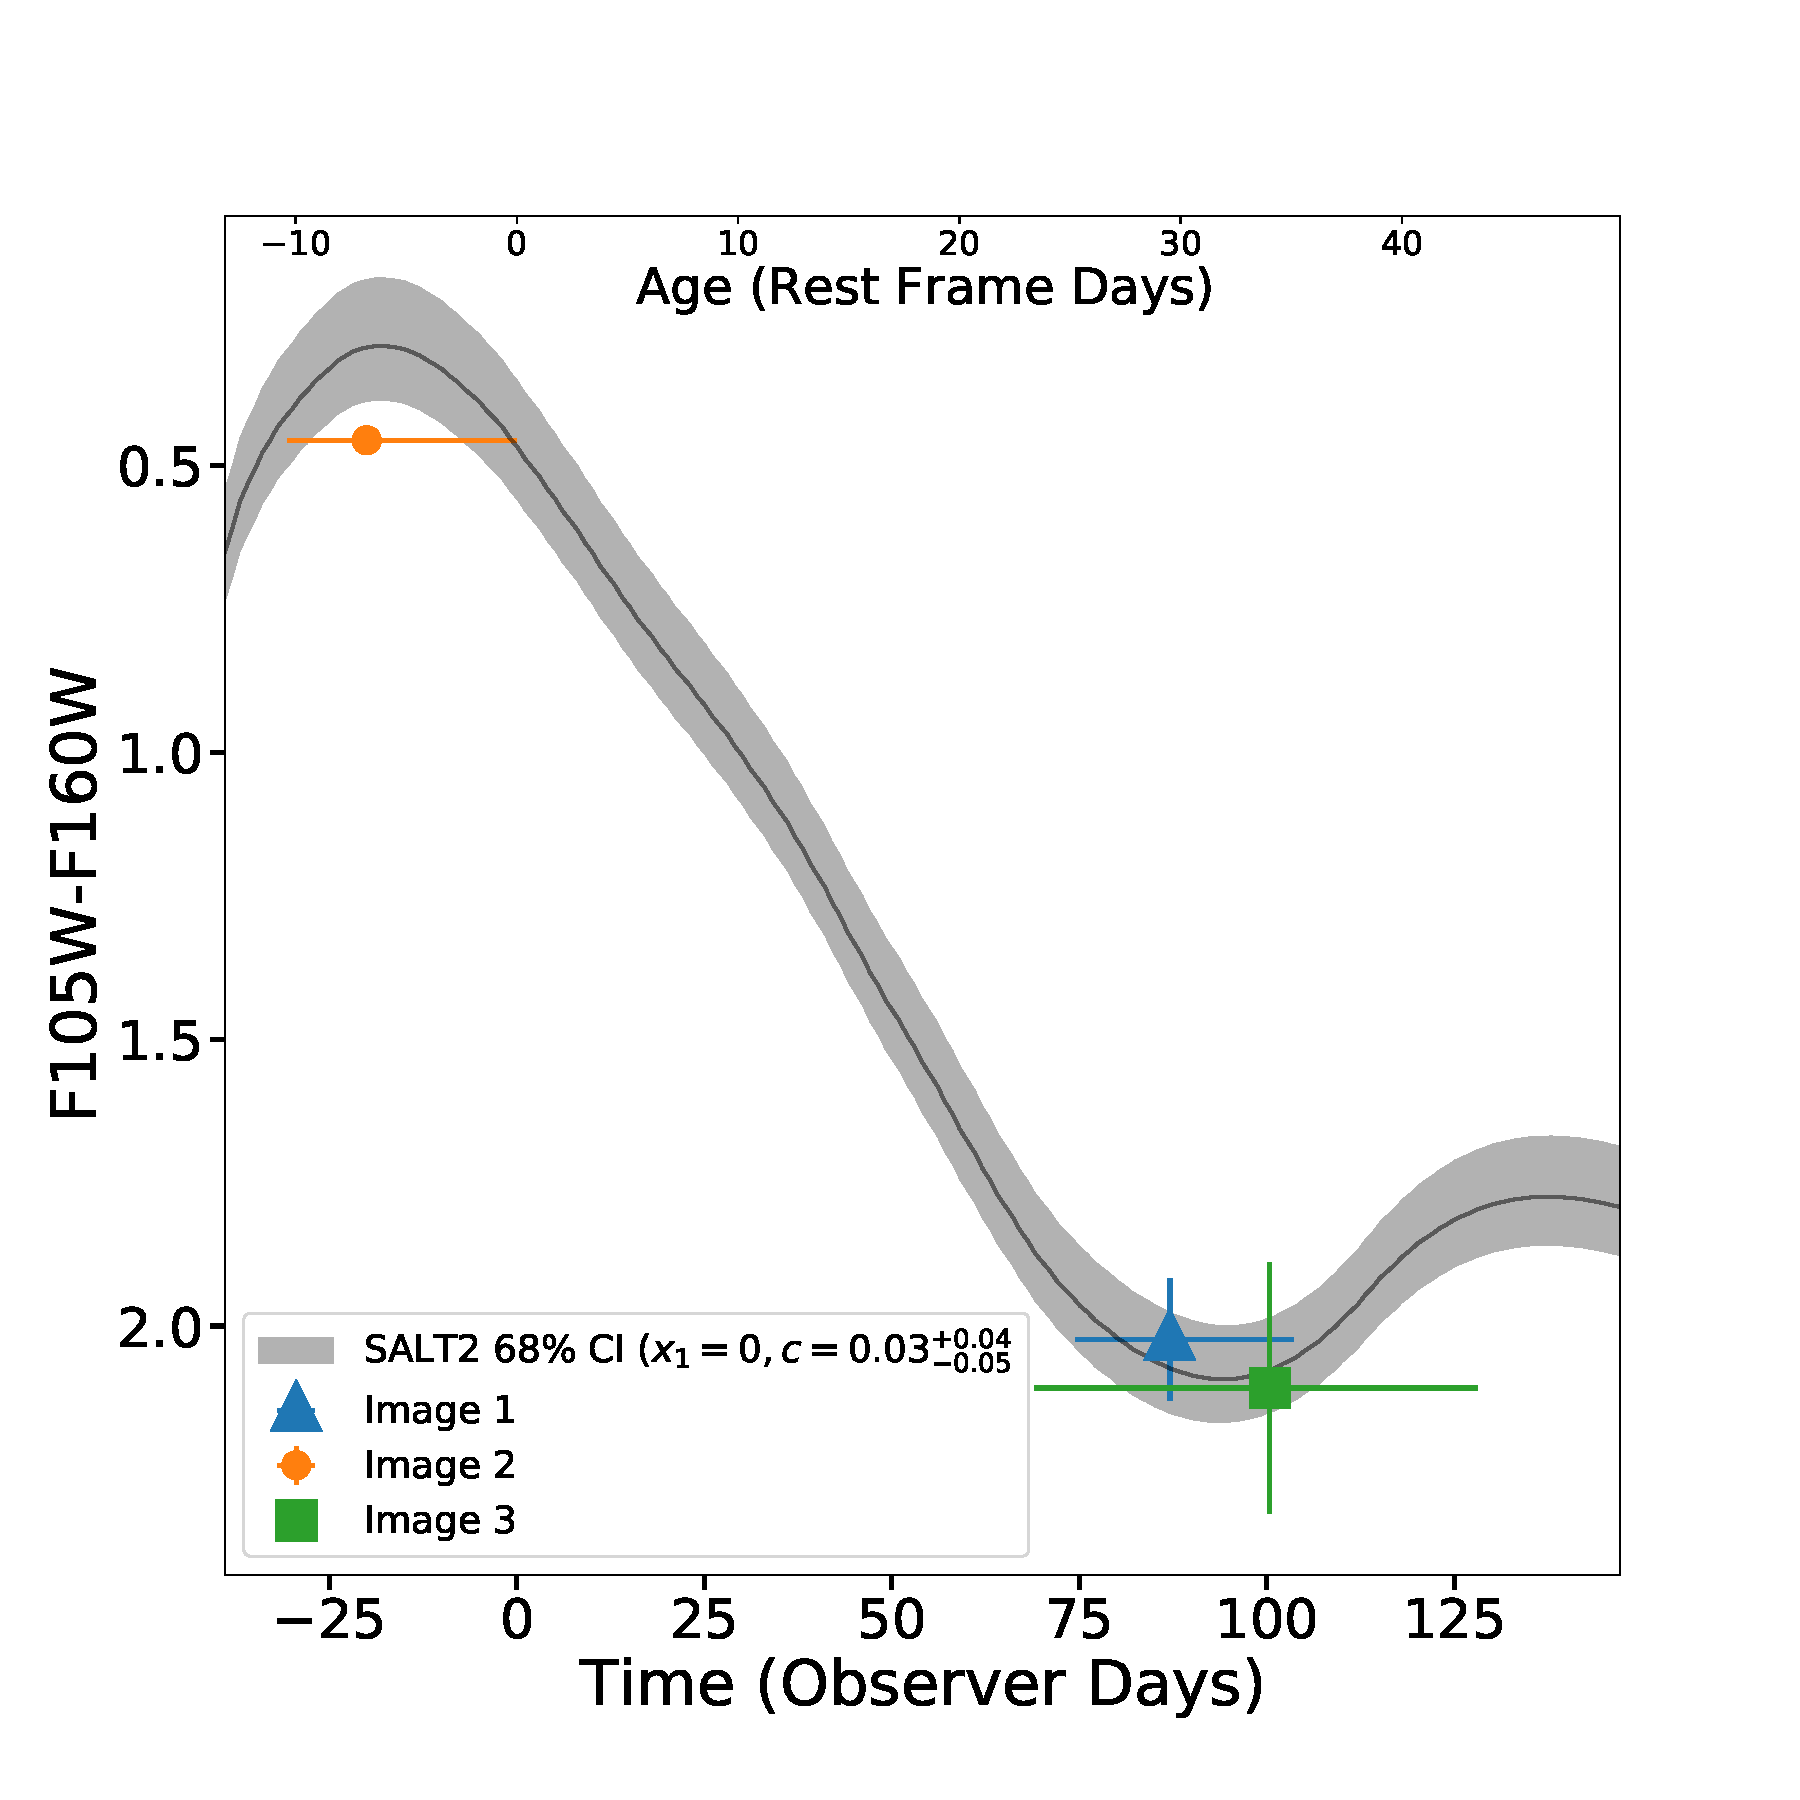
\includegraphics[width=\textwidth]{Paper/Figures/full_colorcurve_total.pdf}
    \caption{\label{fig:full_colorcurve}}
\end{figure}
\clearpage
\section*{References}
\end{document}
















